\chapter{Unsupervised Learning（非监督学习）}

% ============ §14.1 Introduction ============
\section{引言}

\begin{remark}[监督学习回顾]
前面各章处理的都是\textbf{监督学习}：给定输入 $X^T=(X_1,\dots,X_p)$，预测输出 $Y=(Y_1,\dots,Y_m)$。训练样本 $(x_1,y_1),\dots,(x_N,y_N)$ 中联合值全部已知，目标由损失函数 $L(y,\hat y)$（例如平方损失 $(y-\hat y)^2$）刻画。若视 $(X,Y)$ 服从联合密度 $\Pr(X,Y)$，则监督学习本质上是在估计\textbf{条件密度} $\Pr(Y\mid X)$ 的性质，其中最典型的是逐点最小化期望误差的「位置」参数
\begin{equation}
\mu(x) = \argmin_{\theta}\; \E_{Y\mid X} L(Y,\theta). \label{eq:14_1}
\end{equation}
由于 $Y$ 通常低维（一般一维）且只关心位置 $\mu(x)$，加上 $\Pr(X)$（输入的边际密度）在监督学习中一般不是直接关心的对象，问题被大大简化。
\end{remark}

本章转向\textbf{非监督学习}（unsupervised learning，即「无师学习」）。此时只有 $N$ 个观测 $x_1,x_2,\dots,x_N$，来自随机 $p$ 维向量 $X$ 的联合密度 $\Pr(X)$；目标是在\textbf{没有监督者}提供正确解答或误差度量的情况下，直接推断该密度 $\Pr(X)$ 的性质。

与监督学习相比，非监督学习有两个不利因素：
\begin{enumerate}[itemsep=1pt]
\item $X$ 的维数常常\textbf{高得多}；
\item 感兴趣的性质往往比简单的位置估计\textbf{更复杂}。
\end{enumerate}
但也有一点缓解：$X$ 涵盖了所有变量，无需推断 $\Pr(X)$ 的性质如何随另一组变量变化。

在低维情形（$p\le 3$），有各种有效的\textbf{非参数方法}可直接在全体 $X$ 值上估计 $\Pr(X)$ 并作图（Silverman, 1986）。由于\textbf{维数灾难}，这些方法在高维失效，只能退而估计较粗糙的全局模型，如\textbf{高斯混合}或各种刻画 $\Pr(X)$ 的简单描述性统计。一般地，这些描述性统计试图刻画 $\Pr(X)$ 相对较大的那些 $X$ 值或值的集合：

\begin{description}[itemsep=1pt]
\item[主成分、多维缩放（MDS）、自组织映射（SOM）、主曲线]：识别 $X$ 空间中代表高数据密度的一类\textbf{低维流形}，提供变量间关联的信息，以及各变量能否视为少数「隐变量」的函数；
\item[聚类分析]：寻找 $X$ 空间中含 $\Pr(X)$ 众数的\textbf{多个凸区域}，判断 $\Pr(X)$ 是否能表示为若干更简单密度（代表不同类型/类别观测）的混合；
\item[混合建模]：目标与聚类类似；
\item[关联规则]：在极高维\textbf{二元值}数据的特殊情形下，构造描述高密度区域的简单合取规则。
\end{description}

\begin{remark}[非监督学习没有直接的成功度量]
监督学习有清晰的成败度量（联合分布上的期望损失，可用交叉验证估计）；非监督学习\textbf{没有}这种直接度量，很难判定推断的有效性，只能诉诸启发式论证——不仅用于动机，也用于判断结果质量。这种困境导致方法大量涌现，因为「有效性」是见仁见智、无法直接验证的。本章只介绍实践中用得最多的技术，外加作者偏爱的一些方法。
\end{remark}

% ============ §14.2 Association Rules ============
\section{关联规则}

关联规则分析（association rule analysis）已成为挖掘商业数据库的流行工具，目标是找出变量 $X=(X_1,X_2,\dots,X_p)$ 在数据库中出现\textbf{最频繁}的联合取值。它最常应用于二元数据 $X_j\in\{0,1\}$，此时称为\textbf{「市场篮子」分析}（market basket analysis）：观测是销售交易（如收银台结账记录），变量是商店所有商品——$x_{ij}=1$ 表示第 $i$ 笔交易购买了第 $j$ 件商品，否则为 0。经常同时取 1 的变量对应\textbf{经常被一起购买}的商品，可用于货架摆放、交叉营销、目录设计、按购买习惯细分顾客等。

更一般地，关联规则分析的基本目标是找特征向量 $X$ 的一组原型值 $v_1,\dots,v_L$，使密度在这些值处相对较大，即 $\Pr(v_l)$ 相对大。该框架可视为「\textbf{众数寻找}」（mode finding）或「\textbf{凸包搜索}」（bump hunting）。然而这个一般问题极其困难：$\Pr(v_l)$ 的自然估计是 $X=v_l$ 的观测比例，但变量一多、取值一多，$X=v_l$ 的观测数几乎总少到无法可靠估计。因此必须对分析目标与数据普遍性做大幅简化。

\begin{definition}[合取规则]
第一个简化修改目标：不再寻找 $\Pr(x)$ 大的点 $x$，而是寻找 $X$ 空间中\textbf{概率含量相对其尺寸或支撑}较大的区域。设 $S_j$ 为第 $j$ 个变量的全部可能取值（其支撑），$s_j\subseteq S_j$ 为其子集。修改后的目标是找变量取值子集 $s_1,\dots,s_p$，使各变量\textbf{同时}落入相应子集的概率
\begin{equation}
\Pr\left[\bigcap_{j=1}^{p} (X_j\in s_j)\right] \label{eq:14_2}
\end{equation}
相对较大。交集 $\bigcap_{j=1}^{p} (X_j\in s_j)$ 称为一个\textbf{合取规则}（conjunctive rule）。定量变量的 $s_j$ 取\textbf{连续区间}，分类变量的 $s_j$ 显式划定。若 $s_j=S_j$（整个取值集合，常见情形），则称变量 $X_j$ \textbf{不出现}在该规则中。
\end{definition}

\begin{remark}[几何视角：盒子的连续性与分块]
在几何上，合取规则 \eqref{eq:14_2} 是一个\textbf{轴平行、连通}的超矩形（box）：对每个定量坐标取一个连续区间，故单个规则是「连续」的、\textbf{不可分块}。若高密度区域是\textbf{分块/非凸}的（如图 \ref{fig:14_1} 左图的 $2\times 2$ 块），单条规则无法刻画，需用\textbf{多条规则（多个盒子）的并集}来覆盖——这正是「众数寻找 / bump hunting」的思路。此外注意目标是「概率含量\textbf{相对其尺寸}较大」的区域，而非绝对概率 $\Pr(x)$ 最大的点。
\end{remark}

% ============ §14.2.1 Market Basket Analysis ============
\subsection{市场篮子分析}

求解 \eqref{eq:14_2} 的一般方法在 §14.2.5 讨论，对许多应用很有用；但对市场篮子分析常面对的极大数据库（$p\approx 10^4,\ N\approx 10^8$）不可行，还需进一步简化：

\begin{enumerate}[itemsep=1pt]
\item 只考虑\textbf{两种}子集：$s_j$ 为单个值 $\{v_j^0\}$，或为全部取值 $S_j$。于是问题化为找整数子集 $J\subset\{1,\dots,p\}$ 及对应值 $v_j^0\ (j\in J)$，使
\begin{equation}
\Pr\left[\bigcap_{j\in J} (X_j = v_j^0)\right] \label{eq:14_3}
\end{equation}
较大。图 \ref{fig:14_1} 说明了这一假设。
\item 用\textbf{哑变量}技巧把 \eqref{eq:14_3} 转化为纯二元问题。这里 $S_j$ 是 $X_j$ 的\textbf{支撑}（support），即其全部可能取值的集合，假设每个 $S_j$ 有限。\textbf{严格定义}：对每个变量 $X_j$ 的每个取值 $v_l^j\in S_j$，构造一个哑变量 $Z_k$，它是该取值事件的\textbf{指示函数}
\[
Z_k = I(X_j = v_l^j) = \begin{cases} 1, & X_j = v_l^j,\\ 0, & \text{否则}, \end{cases}
\]
其中下标 $k$ 遍历所有 $(j,l)$ 对，故哑变量总数恰为所有变量取值个数之和
\[
K = \sum_{j=1}^{p} |S_j|,
\]
即「把全部变量的所有取值摊平成一条 0/1 向量」的长度。于是 \eqref{eq:14_3} 化为找\textbf{下标集} $\mathcal{K}\subset\{1,\dots,K\}$（花体 $\mathcal{K}$ 区别于哑变量总数 $K$）使
\begin{equation}
\Pr\left[\bigcap_{k\in\mathcal{K}} (Z_k=1)\right] = \Pr\left[\prod_{k\in\mathcal{K}} Z_k = 1\right] \label{eq:14_4}
\end{equation}
较大——这就是市场篮子问题的\textbf{标准形式}。等号成立是因为每个 $Z_k\in\{0,1\}$：「所有 $Z_k$ 都等于 1」当且仅当「其乘积等于 1」，交与乘积只是记号等价。
\end{enumerate}

\begin{figure}[htbp]
\centering
\begin{tikzpicture}[>=stealth, font=\small, scale=1.0]
  % 左面板：2x2 高密度块（无法用单值/全集表示）
  \begin{scope}[shift={(0,0)}]
    \draw[->] (0,0) -- (0,2.6) node[above]{$X_2$};
    \draw[->] (0,0) -- (3.4,0) node[right]{$X_1$};
    \foreach \x in {0.4,1.3,2.2} \draw (\x,0.06) -- (\x,-0.06);
    \foreach \y in {0.4,1.3,2.2} \draw (0.06,\y) -- (-0.06,\y);
    \fill[red!40] (0.4,0.4) rectangle (2.2,1.3);
    \node[red!70!black] at (1.7,-0.45) {左};
  \end{scope}
  % 中面板：单列高密度（X2 取某值，X1 全域？实际为单列）
  \begin{scope}[shift={(4.2,0)}]
    \draw[->] (0,0) -- (0,2.6) node[above]{$X_2$};
    \draw[->] (0,0) -- (3.4,0) node[right]{$X_1$};
    \foreach \x in {0.4,1.3,2.2} \draw (\x,0.06) -- (\x,-0.06);
    \foreach \y in {0.4,1.3,2.2} \draw (0.06,\y) -- (-0.06,\y);
    \fill[red!40] (0.4,0.4) rectangle (1.3,2.2);
    \node[red!70!black] at (1.7,-0.45) {中};
  \end{scope}
  % 右面板：单值（单格）高密度
  \begin{scope}[shift={(8.4,0)}]
    \draw[->] (0,0) -- (0,2.6) node[above]{$X_2$};
    \draw[->] (0,0) -- (3.4,0) node[right]{$X_1$};
    \foreach \x in {0.4,1.3,2.2} \draw (\x,0.06) -- (\x,-0.06);
    \foreach \y in {0.4,1.3,2.2} \draw (0.06,\y) -- (-0.06,\y);
    \fill[red!40] (0.4,1.3) rectangle (1.3,2.2);
    \node[red!70!black] at (1.7,-0.45) {右};
  \end{scope}
  \node[font=\footnotesize] at (5.5,-1.3) {图 \ref{fig:14_1}：关联规则的简化假设。两个输入 $X_1$、$X_2$ 分别取 4 个与 6 个相异值，红框表示高密度区域。};
\end{tikzpicture}
\caption{关联规则的简化假设：高密度区域只能取「某输入的单值」或「全部值」两种形式。此假设下可以找到中、右两种模式，但找不到左侧的 $2\times 2$ 块模式。}
\label{fig:14_1}
\end{figure}

\begin{example}[市场篮子问题的完整流程演示]
为把 \eqref{eq:14_2}--\eqref{eq:14_4} 的抽象过程串成一条直观的链条，这里给出一个不含数值计算的最小例子。

设一家小超市只卖四种商品：牛奶（M）、面包（B）、鸡蛋（E）、黄油（U）。某一天收银台记录了 5 笔交易（市场篮子）：
\begin{center}
\begin{tabular}{cl}
\toprule
交易 $i$ & 购买的商品 \\
\midrule
1 & 牛奶、面包、鸡蛋 \\
2 & 牛奶、面包 \\
3 & 牛奶、鸡蛋、黄油 \\
4 & 面包、鸡蛋 \\
5 & 牛奶、面包、黄油 \\
\bottomrule
\end{tabular}
\end{center}

\textbf{第 1 步：原始目标}。对应 \eqref{eq:14_2}，目标是在四个商品变量 $X_1,\dots,X_4$（均取值 $\{0,1\}$，1 表示购买）上找取值子集 $s_1,\dots,s_4$，使「各商品同时落入其子集」的概率较大。直觉上，牛奶与面包经常一起出现，就是这类高概率的取值组合。

\textbf{第 2 步：单值/全集简化}。按市场篮子分析的简化，每个 $s_j$ 只允许两种形式：单值 $s_j=\{1\}$（要求购买该商品）或全集 $s_j=\{0,1\}$（不约束该商品）。于是 \eqref{eq:14_2} 化为 \eqref{eq:14_3}：找商品子集 $J\subset\{1,2,3,4\}$，使「$J$ 中所有商品都被购买」的概率较大。

\textbf{第 3 步：哑变量编码}。严格按 \eqref{eq:14_3} 之前的公式，每个原始变量的每个取值对应一个哑变量，故 $K=\sum_{j=1}^{4}|S_j|=4\times 2=8$——每个商品对应「买了」「没买」两个哑变量。但市场篮子分析只关心「买了」（$X_j=1$）这个事件，实践中\textbf{省略「没买」哑变量}，每个商品只保留一个购买指示 $Z_k$（直接取 $X_j$ 本身），实际纳入分析的有效哑变量数为 $p=4$。每笔交易变成一个 0/1 向量：
\begin{center}
\begin{tabular}{cccccc}
\toprule
交易 $i$ & $Z_M$ & $Z_B$ & $Z_E$ & $Z_U$ & 含义 \\
\midrule
1 & 1 & 1 & 1 & 0 & 买了牛奶、面包、鸡蛋 \\
2 & 1 & 1 & 0 & 0 & 买了牛奶、面包 \\
3 & 1 & 0 & 1 & 1 & 买了牛奶、鸡蛋、黄油 \\
4 & 0 & 1 & 1 & 0 & 买了面包、鸡蛋 \\
5 & 1 & 1 & 0 & 1 & 买了牛奶、面包、黄油 \\
\bottomrule
\end{tabular}
\end{center}

\textbf{第 4 步：引出项集与支持度}。现在问题化为 \eqref{eq:14_4}：找哑变量下标集 $\mathcal{K}$，使「$\mathcal{K}$ 中所有哑变量同时为 1」（即这些商品同时被购买）的概率较大。例如「牛奶、面包」对应 $\mathcal{K}=\{Z_M,Z_B\}$，它在 5 笔交易中的出现频率就是该组合的\textbf{支持度} $T(\mathcal{K})$——即下文定义中 \eqref{eq:14_5} 所刻画的对象。此处 $N=5$，有效哑变量数为 4，共有 $2^4=16$ 个可能的项集（若按公式口径 $K=8$ 计入「没买」哑变量则为 $2^8=256$，实践中弃之不用）；实际操作中用支持度阈值 $t$（\eqref{eq:14_6}）筛掉出现太少的组合。

这样一个完整的市场篮子问题就串通了：交易数据 $\to$ 单值/全集简化 $\to$ 哑变量编码 $\to$ 项集与支持度。
\end{example}

\begin{definition}[项集、支持度]
设 $\mathcal{K}$ 为哑变量下标集，称 $\mathcal{K}$ 为一个\textbf{项集}（item set），其中哑变量个数称为其\textbf{大小}（size，不超过 $p$）。\eqref{eq:14_4} 的估计取数据库中含该合取的观测比例：
\begin{equation}
\hat\Pr\left[\prod_{k\in\mathcal{K}} Z_k=1\right] = \frac{1}{N}\sum_{i=1}^{N}\prod_{k\in\mathcal{K}} z_{ik}, \label{eq:14_5}
\end{equation}
其中 $z_{ik}$ 是第 $i$ 个案例的 $Z_k$ 值。上式称为项集 $\mathcal{K}$ 的\textbf{支持度}或\textbf{流行度}（support / prevalence）$T(\mathcal{K})$。满足 $\prod_{k\in\mathcal{K}} z_{ik}=1$ 的观测 $i$ 称\textbf{包含}（contain）项集 $\mathcal{K}$。

关联规则挖掘中指定支持度下界 $t$，寻找可由 $Z_1,\dots,Z_K$ 构成、且在数据库中支持度超过 $t$ 的所有项集：
\begin{equation}
\{\mathcal{K}_l \mid T(\mathcal{K}_l) > t\}. \label{eq:14_6}
\end{equation}
\end{definition}

% ============ §14.2.2 The Apriori Algorithm ============
\subsection{Apriori 算法}

只要把阈值 $t$ 调得使 \eqref{eq:14_6} 只占全部 $2^K$ 个项集的很小一部分，\textbf{Apriori 算法}（Agrawal et al., 1995）就能以少量数据遍历求解 \eqref{eq:14_6}。它利用了「维数灾难」的几个方面：对给定支持度阈值 $t$，
\begin{enumerate}[itemsep=1pt]
\item 基数 $|\{\mathcal{K}\mid T(\mathcal{K})>t\}|$ 相对较小；
\item \textbf{单调性}：$\mathcal{K}$ 的任意子集项集 $L$ 的支持度不小于 $\mathcal{K}$ 的，即
\[
L\subseteq \mathcal{K} \;\Longrightarrow\; T(L)\ge T(\mathcal{K}).
\]
\end{enumerate}

\begin{remark}[单调性为什么成立]
直观上，项集越大要求「同时成立」的条件越多、越严格，能同时满足的观测只会更少。严格证明：记包含项集 $\mathcal{K}$ 的观测集合
\[
A(\mathcal{K}) = \left\{ i : \prod_{k\in\mathcal{K}} z_{ik} = 1 \right\},
\]
由 \eqref{eq:14_5} 有 $T(\mathcal{K}) = |A(\mathcal{K})|/N$。若 $L\subseteq\mathcal{K}$，则任何包含 $\mathcal{K}$ 的观测 $i$ 对所有 $k\in\mathcal{K}$ 满足 $z_{ik}=1$，特别地对 $L$ 中所有 $k$ 亦然，故 $i$ 必包含 $L$，从而
\[
A(\mathcal{K})\subseteq A(L) \quad\Longrightarrow\quad T(\mathcal{K})\le T(L).
\]
即「满足更多约束」的观测集合是「满足更少约束」观测集合的子集。例如在 §14.2.1 的市场篮子例子中，$T(\{\text{牛奶}\})=4/5\ge T(\{\text{牛奶,面包}\})=3/5$。

由此得到\textbf{反单调性/向下闭包}（anti-monotone / downward closure）：若 $m$ 项集 $\mathcal{K}$ 不频繁（$T(\mathcal{K})\le t$），则其一切超集也\textbf{不可能频繁}。这正是 Apriori 剪枝的依据：第 $m$ 遍只须考虑「所有 $m-1$ 个祖先项集都频繁」的候选，含非频繁子集的候选可直接丢弃、无需扫描数据。
\end{remark}

\begin{algorithm}[H]
\caption{Apriori 算法（市场篮子）}
\begin{algorithmic}[1]
\Require 事务数据库 $D$（$N$ 笔交易，哑变量 $Z_1,\dots,Z_K$）；最小支持度阈值 $t$
\Ensure 所有频繁项集 $\{\mathcal{K}\mid T(\mathcal{K})>t\}$
\State 扫描 $D$，按 \eqref{eq:14_5} 统计每个单项集支持度，得频繁 $1$-项集 $F_1=\{\{k\}\mid T(\{k\})>t\}$，令 $m\leftarrow 1$
\While{$F_m\neq \varnothing$}
  \State 生成候选 $(m{+}1)$-项集 $C_{m+1}$：由 $F_m$ 中的项集两两合并，且每个候选的所有 $m$-子集都在 $F_m$ 中
  \State 扫描 $D$，统计 $C_{m+1}$ 中每个候选的支持度 $T(\cdot)$
  \State $F_{m+1}\leftarrow\{\mathcal{K}\in C_{m+1}\mid T(\mathcal{K})>t\}$
  \State $m\leftarrow m+1$
\EndWhile
\State \Return $\bigcup_{m\ge 1} F_m$
\end{algorithmic}
\end{algorithm}

\textbf{算法过程（文字描述）}：第一遍遍历数据计算所有\textbf{单项集}的支持度，低于阈值者丢弃；第二遍只计算由第一遍幸存单项构成的两项集，低于阈值者再丢弃；此后每一遍只考虑「由上一遍幸存项集与第一遍保留项组合而成」的候选。生成大小 $m$ 的频繁项集只需考虑其所有 $m-1$ 个祖先项集都频繁的候选。遍历持续到上一遍的候选规则支持度全部低于阈值为止。

关键的一点是：Apriori 对每个 $|K|$ 值\textbf{只需一遍数据}——因为假设数据放不进主存。若数据足够稀疏（或阈值 $t$ 足够高），即使数据集巨大也能在合理时间内终止。Apriori 算法代表了数据挖掘技术的一项重大进步。

\begin{definition}[关联规则及其属性]
每个高支持度项集 $\mathcal{K}$（\eqref{eq:14_6}）被转化为一组\textbf{关联规则}：把 $\mathcal{K}$ 的项划分成两个不相交子集 $A\cup B=\mathcal{K}$，记为
\begin{equation}
A \Rightarrow B. \label{eq:14_7}
\end{equation}
$A$ 称\textbf{前件}（antecedent），$B$ 称\textbf{后件}（consequent）。关联规则有如下性质：
\begin{itemize}[itemsep=1pt]
\item \textbf{支持度} $T(A\Rightarrow B)$：前件与后件并集（即原项集 $\mathcal{K}$）的支持度，可视为随机市场篮子中同时出现 $A$、$B$ 的概率 $\Pr(A\text{ and }B)$ 的估计（\eqref{eq:14_5}）；
\item \textbf{置信度}（或可预测性）$C(A\Rightarrow B)$：支持度除以\textbf{前件}的支持度
\begin{equation}
C(A\Rightarrow B) = \frac{T(A\Rightarrow B)}{T(A)}, \label{eq:14_8}
\end{equation}
可视为 $\Pr(B\mid A)$ 的估计（记号 $\Pr(A)$ 是 $\Pr(\prod_{k\in A}Z_k=1)$ 的简写）；
\item \textbf{期望置信度}（expected confidence）：后件的支持度 $T(B)$，即无条件概率 $\Pr(B)$ 的估计；
\item \textbf{提升度}（lift）：
\[
L(A\Rightarrow B) = \frac{C(A\Rightarrow B)}{T(B)},
\]
即 $\Pr(A \text{ and } B)/[\Pr(A)\Pr(B)]$ 的估计。
\end{itemize}

\medskip
\noindent\textbf{小结}：四种属性的公式、估计对象与常用阈值归纳如下（阈值均为实践常用经验值，需按数据规模与应用调整；其中支持度阈值 $t$、置信度阈值 $c$ 正是 \eqref{eq:14_6}、\eqref{eq:14_9} 中的下界）：
\begin{center}
\begin{tabular}{lcccl}
\toprule
属性 & 记号 & 公式 & 估计对象 & 常用阈值 \\
\midrule
支持度 & $T(A\Rightarrow B)$ & $T(\mathcal{K})$ & $\Pr(A\text{ 且 }B)$ & $t$：$1\%\sim 10\%$ \\
置信度 & $C(A\Rightarrow B)$ & $T(A\Rightarrow B)/T(A)$ & $\Pr(B\mid A)$ & $c$：$50\%\sim 90\%$ \\
期望置信度 & $T(B)$ & $T(B)$ & $\Pr(B)$（基准） & --- \\
提升度 & $L(A\Rightarrow B)$ & $C(A\Rightarrow B)/T(B)$ & $\Pr(A,B)/[\Pr(A)\Pr(B)]$ & $>1$ 正关联，常用 $>1.5$ \\
\bottomrule
\end{tabular}
\end{center}
\end{definition}

\begin{example}[花生酱--果冻--面包]
设项集 $\mathcal{K}=\{\text{peanut butter, jelly, bread}\}$，考虑规则 $\{$peanut butter, jelly$\}\Rightarrow\{\text{bread}\}$。支持度 0.03 表示三种商品同时出现在 3\% 的市场篮子中；置信度 0.82 表示买了花生酱和果冻的篮子里 82\% 也买了面包；若面包出现在 43\% 的篮子中，则该规则提升度为 $1.95$。
\end{example}

\textbf{规则生成}：设置信度阈值 $c$，报告所有由 \eqref{eq:14_6} 的项集构成且置信度超过 $c$ 的规则：
\begin{equation}
\{A\Rightarrow B \mid C(A\Rightarrow B) > c\}. \label{eq:14_9}
\end{equation}
对大小为 $|K|$ 的项集，形如 $A\Rightarrow (K-A),\ A\subset K$ 的规则共有 $2^{|K|-1}-1$ 条。Agrawal 等给出 Apriori 的变体，可快速确定哪些规则通过置信度阈值。

\textbf{整体输出}：满足约束
\[
T(A\Rightarrow B)>t \quad\text{且}\quad C(A\Rightarrow B)>c
\]
的关联规则集合，通常存入可查询的数据库，例如按置信度、提升度或支持度排序展示，或以后件中特定商品为条件筛选——这实际上把问题转入了监督学习框架。

\begin{remark}[关联规则的局限]
关联规则成功的关键是\textbf{支持度阈值}（\eqref{eq:14_6}）保证计算可行。随着该下界减小，解项集的个数、大小以及所需数据遍历次数可能\textbf{指数增长}。因此，高置信度/高提升度但\textbf{低支持度}的规则不会被发现——例如 "vodka $\Rightarrow$ caviar" 这类规则，因后件 caviar 销量低而无法被挖出。
\end{remark}

% ============ §14.2.3 Example: Market Basket Analysis ============
\subsection{示例：市场篮子分析}

我们在中等规模的人口统计数据库上演示 Apriori。数据是旧金山湾区购物中心顾客填写的 $N=9409$ 份问卷（Impact Resources, Inc., Columbus OH, 1987），此处使用前 14 个与人口统计有关的问题（表 \ref{tab:14_1}）。数据是序数变量与（无序）分类变量的混合，很多分类变量取值较多，且含大量缺失值。

\begin{table}[htbp]
\centering
\caption{人口统计数据中的输入变量。}
\label{tab:14_1}
\begin{tabular}{clcl}
\toprule
编号 & 特征 & 取值数 & 类型 \\
\midrule
1  & Sex（性别）               & 2 & 分类 \\
2  & Marital status（婚姻状况） & 5 & 分类 \\
3  & Age（年龄）               & 7 & 序数 \\
4  & Education（教育）         & 6 & 序数 \\
5  & Occupation（职业）        & 9 & 分类 \\
6  & Income（收入）            & 9 & 序数 \\
7  & Years in Bay Area（居留年数） & 5 & 序数 \\
8  & Dual incomes（双收入）    & 3 & 分类 \\
9  & Number in household（家庭人数）& 9 & 序数 \\
10 & Number of children（子女数）& 9 & 序数 \\
11 & Householder status（户主身份）& 3 & 分类 \\
12 & Type of home（住房类型）   & 5 & 分类 \\
13 & Ethnic classification（族裔）& 8 & 分类 \\
14 & Language in home（家庭语言）& 3 & 分类 \\
\bottomrule
\end{tabular}
\end{table}

使用 Christian Borgelt 提供的免费 Apriori 实现（\texttt{http://fuzzy.cs.uni-magdeburg.de/$\sim$borgelt}）。剔除含缺失值的观测后，每个序数预测变量按\textbf{中位数}切分、编码为两个哑变量；每个有 $k$ 类的分类变量编码为 $k$ 个哑变量，最终得到 $6876\times 50$ 的矩阵（6876 个观测、50 个哑变量）。

算法共找到 \textbf{6288} 条关联规则，涉及 $\le 5$ 个预测变量，支持度至少 10\%。理解这大批规则本身就是一项富有挑战性的数据分析任务。图 \ref{fig:14_2}（书中图 14.2）显示了各哑变量在数据中的相对频率（上）与在关联规则中的相对频率（下）：常见类别往往在规则中更频繁出现（如家庭语言的第一类 English），而有些（如 occupation）被低估。

\begin{figure}[htbp]
\centering
\begin{tikzpicture}[>=stealth, font=\small]
  \draw[->] (0,0) -- (0,3.2) node[above]{相对频率};
  \draw[->] (0,0) -- (7,0) node[right]{哑变量序号 $k$};
  \foreach \x/\h in {0.3/1.8,0.8/1.1,1.3/1.4,1.8/1.6,2.3/0.9,2.8/1.2,3.3/0.8,3.8/1.5,4.3/1.0,4.8/1.3,5.3/0.7,5.8/1.1,6.3/1.4}{
    \fill[blue!60!black] (\x,\h) rectangle (\x+0.28,0);
  }
  \node[font=\footnotesize] at (3.5,-0.6) {图 \ref{fig:14_2}（示意）：数据中（上）与规则中（下）各哑变量相对频率的对比};
\end{tikzpicture}
\caption{市场篮子分析（书中图 14.2 的示意）：Apriori 找到的规则中各哑变量（编码一个输入类别）的相对频率。}
\label{fig:14_2}
\end{figure}

书中给出 Apriori 找到的三条示例规则：

\begin{example}[三条示例规则]
\textbf{规则 1}：支持度 25\%，置信度 99.7\%，提升度 1.03。
\[
\left[\begin{array}{c}
\text{number in household}=1\\
\text{number of children}=0
\end{array}\right]
\;\Longrightarrow\;
\text{language in home}=\text{English}.
\]

\textbf{规则 2}：支持度 13.4\%，置信度 80.8\%，提升度 2.13。
\[
\left[\begin{array}{c}
\text{language in home}=\text{English}\\
\text{householder status}=\text{own}\\
\text{occupation}=\{\text{professional/managerial}\}
\end{array}\right]
\;\Longrightarrow\;
\text{income}\ge \$40{,}000.
\]

\textbf{规则 3}：支持度 26.5\%，置信度 82.8\%，提升度 2.15。
\[
\left[\begin{array}{c}
\text{language in home}=\text{English}\\
\text{income}<\$40{,}000\\
\text{marital status}=\text{not married}\\
\text{number of children}=0
\end{array}\right]
\;\Longrightarrow\;
\text{education}\notin\{\text{college graduate, graduate study}\}.
\]
\end{example}

我们根据高支持度选了规则 1 和 3；规则 2 是「高收入」后件的关联规则，可用于定向瞄准高收入人群。

\begin{remark}[哑变量的取舍]
如前所述，每个输入类别都建了哑变量，例如 $Z_1=I(\text{income}<\$40{,}000)$ 与 $Z_2=I(\text{income}\ge \$40{,}000)$。若只关心与「高收入」类别的关联，就只把 $Z_2$ 纳入（而不放 $Z_1$）。实际市场篮子问题常如此：我们关心与\textbf{相对稀有商品的出现}的关联，而不关心与其\textbf{缺失}的关联。
\end{remark}

% ============ §14.2.4 Unsupervised as Supervised Learning ============
\subsection{非监督转化为监督学习}

本节讨论把\textbf{密度估计问题转化为监督函数逼近}的技巧，它是下一节广义关联规则的基础。

\begin{definition}[密度估计转分类]
设 $g(x)$ 为待估计的未知数据密度，$g_0(x)$ 为指定的\textbf{参考密度}（例如变量范围内的均匀密度）。数据 $x_1,\dots,x_N$ 视为来自 $g(x)$ 的 i.i.d. 样本；用 Monte Carlo 方法从 $g_0(x)$ 抽取大小为 $N_0$ 的样本。把两组数据合并，并赋予权重
\[
w = \frac{N_0}{N+N_0}\ (\text{来自 } g),\qquad w_0 = \frac{N}{N+N_0}\ (\text{来自 } g_0),
\]
得到来自\textbf{混合密度} $(g(x)+g_0(x))/2$ 的随机样本。若给来自 $g(x)$ 的样本标 $Y=1$、来自 $g_0(x)$ 的标 $Y=0$，则
\begin{equation}
\mu(x) = \E(Y\mid x) = \frac{g(x)}{g(x)+g_0(x)} = \frac{g(x)/g_0(x)}{1+g(x)/g_0(x)} \label{eq:14_10}
\end{equation}
可用\textbf{监督学习}在合并样本
\begin{equation}
(y_1,x_1), (y_2,x_2), \dots, (y_{N+N_0}, x_{N+N_0}) \label{eq:14_11}
\end{equation}
上估计。所得估计 $\hat\mu(x)$ 可反演为 $g(x)$ 的估计：
\begin{equation}
\hat g(x) = g_0(x)\,\frac{\hat\mu(x)}{1-\hat\mu(x)}. \label{eq:14_12}
\end{equation}
\end{definition}

\begin{example}[一维密度估计转分类的完整流程]
设数据密度为 $g(x)=2x$（$x\in[0,1]$，高密度在右半），参考密度取均匀 $g_0(x)=1$。取 $N_0=N$（两样本等大，使混合严格为等权的 $(g+g_0)/2$；一般 $N_0\neq N$ 时混合密度为加权形式 $[N\,g(x)+N_0\,g_0(x)]/(N+N_0)$，此时 \eqref{eq:14_10} 应代以带权重的 $\mu(x)=N\,g(x)/[N\,g(x)+N_0\,g_0(x)]$）。

\textbf{第 1 步：构造两类样本}。从 $g(x)=2x$ 抽 $N$ 个数据点（大多落在 $x>0.5$ 一侧），标 $Y=1$；从 $g_0(x)=1$ 用 Monte Carlo 抽 $N_0=N$ 个参考点（均匀散布），标 $Y=0$。合并后每点来自混合密度
\[
\frac{g(x)+g_0(x)}{2}=\frac{2x+1}{2}.
\]

\textbf{第 2 步：分类目标}。由 \eqref{eq:14_10}，
\[
\mu(x)=\frac{g(x)}{g(x)+g_0(x)}=\frac{2x}{2x+1},
\]
它是 $x$ 的单调递增曲线：如 $\mu(0.25)=1/3$（更像参考点）、$\mu(0.75)=3/5$（更像数据点）。分类器只需学会这条简单曲线。

\textbf{第 3 步：反演还原}。用 \eqref{eq:14_12}：
\[
\hat g(x)=g_0(x)\,\frac{\hat\mu(x)}{1-\hat\mu(x)}
=\frac{2x/(2x+1)}{1/(2x+1)}=2x=g(x),
\]
精确还原数据密度。若用对数几率 \eqref{eq:14_13} 则 $f(x)=\log[g(x)/g_0(x)]=\log(2x)$，\eqref{eq:14_14} 同样给出 $\hat g=g_0 e^{\hat f}=2x$。

可见：把密度估计「伪装」成分类后，只需拟合 $\mu$（或 $f$）这个简单对象，再经单调反演即得 $\hat g$。
\end{example}

\textbf{广义逻辑回归}（第 4.4 节）尤其适合此应用，因为它直接估计\textbf{对数几率}（log-odds）
\begin{equation}
f(x) = \log\frac{g(x)}{g_0(x)}, \label{eq:14_13}
\end{equation}
此时
\begin{equation}
\hat g(x) = g_0(x)\, e^{\hat f(x)}. \label{eq:14_14}
\end{equation}

\begin{example}[书中图 14.3：通过分类进行密度估计]
\begin{figure}[H]
\centering
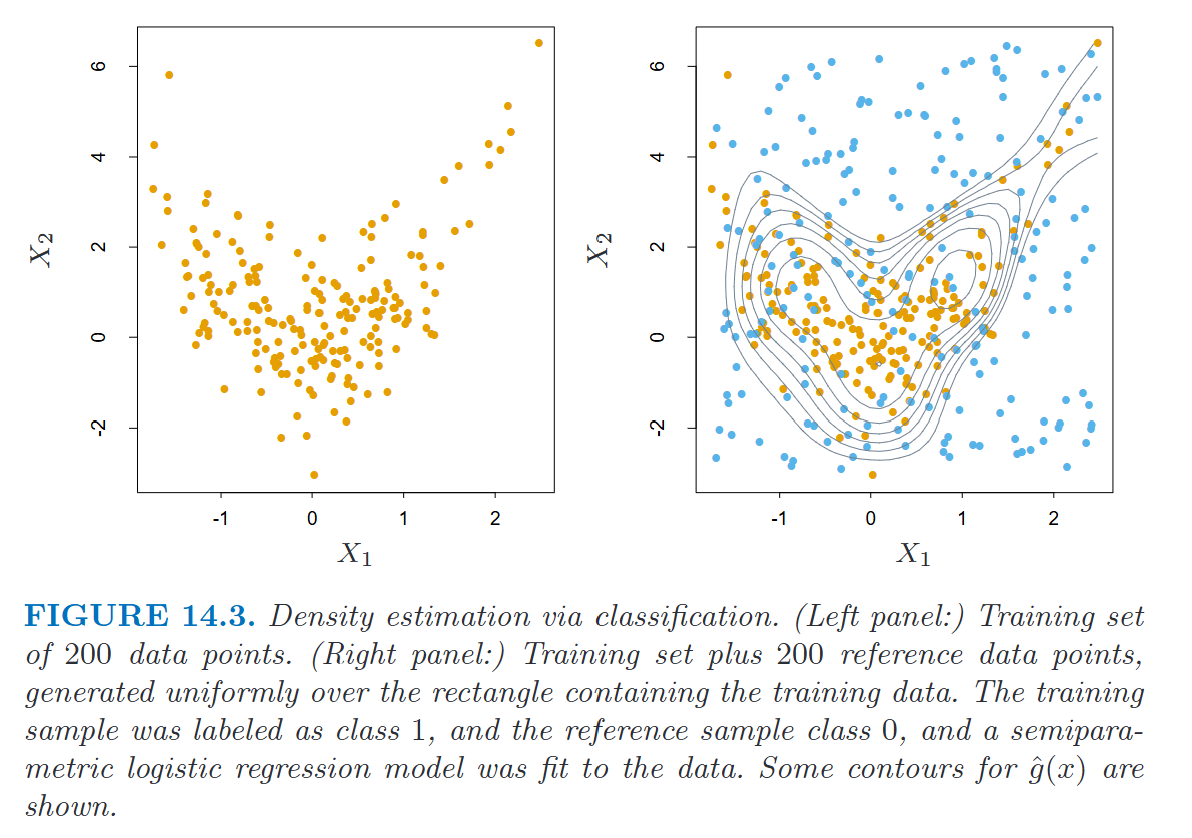
\includegraphics[width=0.95\textwidth]{Chapters/pic/ch_非监督学习/figure_14_3.png}
\caption{通过分类进行密度估计。（左图）训练集 200 个数据点。（右图）训练集加上 200 个参考数据点，参考点在包含训练数据的最小矩形上均匀生成；训练样本标为类 1、参考样本标为类 0，用半参数逻辑回归模型拟合数据，图中显示若干 $\hat g(x)$ 的等值线。}
\label{fig:14_3}
\end{figure}

左图：200 个训练点。右图：在包含训练数据的最小矩形上均匀生成 200 个\textbf{参考点}（蓝色），训练样本标为类 1、参考样本标为类 0，用\textbf{自然样条张量积}的逻辑回归（第 5.2.1 节）拟合。图中显示若干 $\hat\mu(x)$ 的等值线；由于 $\hat g(x)=\hat\mu(x)/(1-\hat\mu(x))$ 是 $\hat\mu$ 的单调函数，这些等值线也是密度估计 $\hat g(x)$ 的等值线，大致刻画了数据密度。
\end{example}

\begin{remark}[参考密度的选择]
原则上 \eqref{eq:14_14} 中 $g_0(x)$ 可取任意参考密度，但实际中 $\hat g(x)$ 的精度可能对 $g_0$ 的选择高度敏感，且取决于数据密度 $g(x)$ 与估计 \eqref{eq:14_10} / \eqref{eq:14_13} 所用的方法。若以精度为目标，应选使 $\mu(x)$ 或 $f(x)$ 易于被所用方法逼近的 $g_0$。

但精度并非总是首要目标：$\mu(x)$ 与 $f(x)$ 都是密度比 $g(x)/g_0(x)$ 的\textbf{单调函数}，可视为「\textbf{对比统计量}」（contrast statistics），提供数据密度 $g$ 偏离所选参考密度 $g_0$ 的信息。因此在数据分析场景中，$g_0$ 的选择由具体问题中\textbf{最感兴趣的偏离类型}决定：
\begin{itemize}[itemsep=1pt]
\item 关心\textbf{偏离均匀}：$g_0$ 取变量范围内的均匀密度；
\item 关心\textbf{偏离联合正态}：$g_0$ 取与数据同均值、同协方差的高斯分布；
\item 研究\textbf{偏离独立}：取
\begin{equation}
g_0(x) = \prod_{j=1}^{p} g_j(x_j), \label{eq:14_15}
\end{equation}
其中 $g_j(x_j)$ 是 $X_j$ 第 $j$ 个坐标的\textbf{边际数据密度}。来自该独立密度 \eqref{eq:14_15} 的样本极易由数据本身生成——只需对各变量的数据值施加\textbf{不同的随机置换}。
\end{itemize}
\end{remark}

\begin{remark}[此法为何未被重视]
这种把问题转化为监督学习（\eqref{eq:14_10}--\eqref{eq:14_14}）的思路似乎是统计学中的「民间传说」，但至今影响不大。原因之一：问题需用 Monte Carlo \textbf{模拟数据集}扩充，且该数据集至少不小于原始样本（$N_0\ge N$），计算与内存需求至少翻倍；生成 Monte Carlo 样本本身也需要大量计算。随着计算资源日益廉价，这一障碍正变得越来越小。
\end{remark}

% ============ §14.2.5 Generalized Association Rules ============
\subsection{广义关联规则}

更一般的寻找高密度区域问题 \eqref{eq:14_2} 可用上述\textbf{监督学习途径}解决。虽然它不适用于市场篮子分析那种巨型数据库，但能从中等规模数据集中获得有用信息。\eqref{eq:14_2} 可表述为：找整数子集 $J\subset\{1,2,\dots,p\}$ 及对应变量 $X_j$ 的取值子集 $s_j\ (j\in J)$，使
\begin{equation}
\hat\Pr\left[\bigcap_{j\in J} (X_j\in s_j)\right] = \frac{1}{N}\sum_{i=1}^{N} I\left[\bigcap_{j\in J} (x_{ij}\in s_j)\right] \label{eq:14_16}
\end{equation}
较大。沿用关联规则分析的术语，$\{(X_j\in s_j)\}_{j\in J}$ 称为一个\textbf{「广义」项集}（generalized item set），定量变量对应的子集 $s_j$ 取其取值范围内的\textbf{连续区间}，分类变量的子集可含\textbf{多于一个值}。

广义表述野心之大，使无法像市场篮子分析那样对支持度（\eqref{eq:14_16}）超过指定下界的\textbf{所有}广义项集穷举搜索，只能用\textbf{启发式搜索}，最多期望找到一组有用的广义项集。

\begin{remark}[均匀分布的隐含偏好]
市场篮子分析（\eqref{eq:14_5}）与广义表述（\eqref{eq:14_16}）都\textbf{隐含参照均匀分布}：寻找「比所有联合取值均匀分布时更频繁」的项集。这偏向发现\textbf{边际成分本身频繁}的项集，即
\begin{equation}
\frac{1}{N}\sum_{i=1}^{N} I(x_{ij}\in s_j) \label{eq:14_17}
\end{equation}
较大。频繁子集（\eqref{eq:14_17}）的合取会比边际较不频繁子集的合取更常出现在高支持度项集（\eqref{eq:14_16}）中——这正是 \texttt{vodka} $\Rightarrow$ \texttt{caviar} 难被发现的原因：二者边际支持度都不高，联合支持度尤其小。参照均匀分布还会使「成分间关联弱但自身高频」的项集主导最高支持度项集的集合。

用边际密度的乘积（\eqref{eq:14_15}）作参考分布可\textbf{消除}对高频单值的偏好：因为若变量间完全独立，密度比 $g(x)/g_0(x)$ 恰为常数（均匀），与各变量取值的频率分布无关，于是 \texttt{vodka} $\Rightarrow$ \texttt{caviar} 这类规则有机会浮现。但如何把均匀之外的参考分布纳入 Apriori 尚不明确；不过按 §14.2.4，从乘积密度 \eqref{eq:14_15} 生成样本是容易的。
\end{remark}

选定参考分布并按 \eqref{eq:14_11} 抽取样本后，就得到一个输出为二值 $Y\in\{0,1\}$ 的\textbf{监督学习问题}。目标是用这些训练数据寻找目标函数 $\mu(x)=\E(Y\mid x)$ 相对较大的\textbf{区域}
\begin{equation}
R = \bigcap_{j\in J} (X_j\in s_j), \label{eq:14_18}
\end{equation}
并且可能还要求这些区域的数据支持
\begin{equation}
T(R) = \int_{x\in R} g(x)\,dx \label{eq:14_19}
\end{equation}
不过小。

% ============ §14.2.6 Choice of Supervised Learning Method ============
\subsection{监督学习方法的选择}

区域（\eqref{eq:14_18}）由合取规则定义，因此\textbf{能学习此类规则}的监督方法最合适。

\textbf{CART 决策树}：其终结点正由形如 \eqref{eq:14_18} 的规则定义。把 CART 应用于合并数据（\eqref{eq:14_11}），将得到一棵在整个数据空间上用一组\textbf{不相交区域}（终结点）建模目标（\eqref{eq:14_10}）的决策树。平均 $y$ 值
\[
\bar y_t = \mathrm{ave}(y_i \mid x_i \in t)
\]
较高的终结点 $t$ 就是高支持度广义项集（\eqref{eq:14_16}）的候选，其（数据）支持度为
\[
T(R) = \bar y_t \cdot \frac{N_t}{N+N_0},
\]
其中 $N_t$ 是该终结点区域内（合并）观测的个数。检查所得决策树可发现相对高支持度的有趣广义项集，再把它们划分成前件与后件，搜索高置信度/高提升度的广义关联规则。

\textbf{PRIM}（第 9.3 节）是另一种自然选择：它也产生形如 \eqref{eq:14_18} 的规则，但\textbf{专门设计用于寻找区域内部平均目标（\eqref{eq:14_10}）最大的高支持度区域}，而非对整个数据空间建模目标函数；它还对「支持度 vs 平均目标值」的权衡提供更多控制。

练习 14.3 讨论这两种方法在从边际分布乘积生成随机数据时的一个问题。

% ============ §14.2.7 Example: Market Basket Analysis (Continued) ============
\subsection{示例：市场篮子分析（续）}

把 PRIM 应用于表 \ref{tab:14_1} 的人口统计数据，得到三个高支持度广义项集：

\begin{example}[PRIM 得到的三个广义项集]
\textbf{项集 1}（支持度 24\%）：
\[
\left[\begin{array}{c}
\text{marital status}=\text{married}\\
\text{householder status}=\text{own}\\
\text{type of home}\ne\text{apartment}
\end{array}\right]
\]

\textbf{项集 2}（支持度 24\%）：
\[
\left[\begin{array}{c}
\text{age}\le 24\\
\text{marital status}\in\{\text{living together-not married, single}\}\\
\text{occupation}\notin\{\text{professional, homemaker, retired}\}\\
\text{householder status}\in\{\text{rent, live with family}\}
\end{array}\right]
\]

\textbf{项集 3}（支持度 15\%）：
\[
\left[\begin{array}{c}
\text{householder status}=\text{rent}\\
\text{type of home}\ne\text{house}\\
\text{number in household}\le 2\\
\text{number of children}=0\\
\text{occupation}\notin\{\text{homemaker, student, unemployed}\}\\
\text{income}\in[\$20{,}000,\ \$150{,}000]
\end{array}\right]
\]
\end{example}

由这些项集派生出置信度（\eqref{eq:14_8}）大于 95\% 的广义关联规则：

\begin{example}[置信度 $>95\%$ 的广义关联规则]
\textbf{规则 1}：支持度 25\%，置信度 99.7\%，提升度 1.35。
\[
\{\text{marital status}=\text{married},\ \text{householder status}=\text{own}\}
\;\Rightarrow\;
\text{type of home}\ne\text{apartment}.
\]

\textbf{规则 2}：支持度 25\%，置信度 98.7\%，提升度 1.97。
\[
\{\text{age}\le 24,\ \text{occupation}\notin\{\text{professional, homemaker, retired}\},\ \text{householder status}\in\{\text{rent, live with family}\}\}
\;\Rightarrow\;
\text{marital status}\in\{\text{single, living together-not married}\}.
\]

\textbf{规则 3}：支持度 25\%，置信度 95.9\%，提升度 2.61。
\[
\{\text{householder status}=\text{own},\ \text{type of home}\ne\text{apartment}\}
\;\Rightarrow\;
\text{marital status}=\text{married}.
\]

\textbf{规则 4}：支持度 15\%，置信度 95.4\%，提升度 1.50。
\[
\{\text{householder status}=\text{rent},\ \text{type of home}\ne\text{house},\ \text{number in household}\le 2,\ \text{occupation}\notin\{\text{homemaker, student, unemployed}\},\ \text{income}\in[\$20{,}000,\$150{,}000]\}
\;\Rightarrow\;
\text{number of children}=0.
\]
\end{example}

这些规则没有大的意外，大多验证了直觉；但在先验信息较少的其他场景中，意外结果更可能涌现。它们展示了广义关联规则能提供的信息类型，以及「监督学习途径 + CART/PRIM 等规则归纳方法」能发现成分间高关联的项集。

\begin{remark}[Apriori 与 PRIM 的对比]
Apriori 是\textbf{穷举}的——找出所有支持度超过给定值的规则；PRIM 是\textbf{贪婪}的，不保证给出「最优」规则集。另一方面，Apriori 只能处理\textbf{哑变量}，因而找不到上述某些规则：例如 \texttt{type of home} 是分类输入、每个水平一个哑变量，Apriori 无法找到涉及集合 $\{\text{type of home}\ne\text{apartment}\}$ 的规则（除非预先为「apartment vs 其他」编码哑变量）；而预先编码所有这类潜在有趣的比较通常不可行。
\end{remark}

% ============ §14.3 Cluster Analysis ============
\section{聚类分析}

聚类分析（cluster analysis），又称\textbf{数据分割}（data segmentation），有一系列目标，都与把对象集合划分成子集或「簇」有关：使同一簇内的对象彼此比不同簇的对象\textbf{更相似}。对象可由一组测量描述，也可由其与其他对象的关系描述。有时目标还包括把簇组织成\textbf{自然层次}——逐层对簇本身再分组，使层次每一层中同一组的簇比不同组的更相似。聚类分析也用于形成描述性统计，判断数据是否由若干性质显著不同的子群组成（这需要评估分到各簇的对象间的差异程度）。

\begin{remark}[相似度量的核心地位]
聚类分析所有目标的核心是对象间的\textbf{相似度/不相似度}（similarity / dissimilarity）概念。聚类方法基于提供给它的相似度定义来分组，而这种定义只能来自\textbf{领域知识}——类似监督学习中损失/代价函数的选择（那里不准确预测的代价取决于数据之外的考量）。
\end{remark}

图 \ref{fig:14_4} 展示了用流行的 K-means 算法把模拟数据聚成三簇（橙色、蓝色、绿色）的例子。其中两簇\textbf{分离不好}，用「分割」比「聚类」更贴切。K-means 从三个簇中心的猜测出发，然后交替以下两步直到收敛：
\begin{enumerate}[itemsep=1pt]
\item 对每个数据点，找出\textbf{欧氏距离}最近的簇中心；
\item 把每个簇中心替换为所有离它最近数据点的\textbf{坐标平均}。
\end{enumerate}
K-means 是\textbf{自上而下}（top-down）的过程，而后面讨论的其他聚类方法是\textbf{自下而上}（bottom-up）的。所有聚类技术的基础是两对象间\textbf{距离/不相似度量}的选择——先讨论距离度量，再描述各类聚类算法。

\begin{figure}[htbp]
\centering
\begin{tikzpicture}[>=stealth, font=\small, scale=1.0]
  % 三个簇示意
  \foreach \x/\y in {1.0/1.2,1.3/1.5,0.9/1.7,1.5/1.3,1.2/1.9,1.7/1.8,1.0/1.4}{
    \fill[orange] (\x,\y) circle (2pt);
  }
  \foreach \x/\y in {3.2/3.4,3.5/3.1,3.8/3.6,3.3/3.8,3.9/3.3,3.6/3.5,4.1/3.2}{
    \fill[blue!70!black] (\x,\y) circle (2pt);
  }
  \foreach \x/\y in {3.1/1.1,3.4/1.4,3.7/1.2,3.3/1.7,3.9/1.5,3.6/1.3,4.0/1.8}{
    \fill[green!55!black] (\x,\y) circle (2pt);
  }
  \draw[->] (0,0) -- (0,4.6) node[above]{$X_2$};
  \draw[->] (0,0) -- (4.8,0) node[right]{$X_1$};
\end{tikzpicture}
\caption{K-means 聚类（书中图 14.4 的示意）：模拟数据被聚成三类（橙、蓝、绿），其中两类分离得不好，「分割」比「聚类」更贴切。}
\label{fig:14_4}
\end{figure}

% ============ §14.3.1 Proximity Matrices ============
\subsection{邻近矩阵}

有时数据直接以对象对的\textbf{邻近度}（proximity，相似或亲和）表示，可以是相似度或不相似度。例如社会科学实验中让参与者判断某些对象彼此差异多大，再对这些判断取平均得到不相似度。这类数据可表示为 $N\times N$ 矩阵 $D$（$N$ 为对象数），元素 $d_{ii'}$ 记录第 $i$ 与第 $i'$ 个对象间的邻近度，直接作为聚类算法的输入。

多数算法假定不相似度矩阵满足\textbf{非负}、\textbf{零对角}（$d_{ii}=0$）。若原始数据是相似度，可用合适的\textbf{单调递减函数}转为不相似度。多数算法还假定矩阵\textbf{对称}；若不满足，用 $(D+D^T)/2$ 代替。主观判断的不相似度通常\textbf{不是严格意义}的距离——三角不等式 $d_{ii'}\le d_{ik}+d_{i'k}$ 未必成立，因此某些假设距离的算法不能用于这类数据。

% ============ §14.3.2 Dissimilarities Based on Attributes ============
\subsection{基于属性的不相似性}

最常见的情形是有 $N$ 个观测、$p$ 个变量（属性）的测量 $x_{ij}$。多数流行聚类算法以不相似度矩阵为输入，故须先构造观测对间的不相似度。通常定义第 $j$ 个属性值间的不相似度 $d_j(x_{ij},x_{i'j})$，再定义对象 $i$ 与 $i'$ 间的
\begin{equation}
D(x_i,x_{i'}) = \sum_{j=1}^{p} d_j(x_{ij},x_{i'j}), \label{eq:14_20}
\end{equation}
最常见的取\textbf{平方距离}
\begin{equation}
d_j(x_{ij},x_{i'j}) = (x_{ij}-x_{i'j})^2. \label{eq:14_21}
\end{equation}
但其他选择也可能且会带来不同结果；对非定量属性（如分类数据）平方距离未必合适；有时还希望给属性\textbf{不同权重}而非如 \eqref{eq:14_20} 的等权。

按属性类型讨论：
\begin{description}[itemsep=1pt]
\item[定量变量]：取值是连续实数，自然的「误差」是绝对差值的单调增函数
\[
d(x_i,x_{i'}) = l(|x_i-x_{i'}|).
\]
除平方误差 $(x_i-x_{i'})^2$ 外，常用恒等（绝对误差），前者更强调较大差异。也可基于\textbf{相关}
\begin{equation}
\rho(x_i,x_{i'}) = \frac{\sum_j (x_{ij}-\bar x_i)(x_{i'j}-\bar x_{i'})}{\sqrt{\sum_j (x_{ij}-\bar x_i)^2\,\sum_j (x_{i'j}-\bar x_{i'})^2}}, \label{eq:14_22}
\end{equation}
其中 $\bar x_i=\sum_j x_{ij}/p$（注意是对\textbf{变量}平均而非观测）。若先把观测标准化，则 $\sum_j(x_{ij}-x_{i'j})^2\propto 2(1-\rho(x_i,x_{i'}))$，故基于相关（相似度）的聚类与基于平方距离（不相似度）的聚类等价。
\item[序数变量]：取值常表示为连续整数、构成有序集（如成绩 A,B,C,D,F）。其误差度量一般先把 $M$ 个原始值按原顺序替换为
\begin{equation}
\frac{i-\frac12}{M},\quad i=1,\dots,M \label{eq:14_23}
\end{equation}
再按此尺度当定量变量处理。秩数据是序数数据的特例。
\item[分类变量]：对无序分类（nominal）变量，值对间的差异程度须显式划定。若变量取 $M$ 个相异值，可排成对称 $M\times M$ 矩阵，元素满足 $L_{rr'}=L_{r'r},\ L_{rr}=0,\ L_{rr'}\ge 0$。最常见取 $L_{rr'}=1$（$r\ne r'$）；也可用不等损失强调某些错误。
\end{description}

% ============ §14.3.3 Object Dissimilarity ============
\subsection{对象不相似性}

把 $p$ 个属性的不相似度 $d_j(x_{ij},x_{i'j})$ 合并成两个对象 $x_i,x_{i'}$ 间整体不相似度的过程，几乎总是用\textbf{加权平均（凸组合）}
\begin{equation}
D(x_i,x_{i'}) = \sum_{j=1}^{p} w_j\cdot d_j(x_{ij},x_{i'j}),\qquad \sum_{j=1}^{p} w_j = 1, \label{eq:14_24}
\end{equation}
其中 $w_j$ 是第 $j$ 个属性的权重，调节它在对象整体不相似度中的相对影响，应基于领域知识选择。

\begin{remark}[等权重不等于等影响]
把 $w_j$ 设为相同值（如 $w_j=1,\ \forall j$）\textbf{并不必然}给所有属性相等影响。第 $j$ 个属性对 $D(x_i,x_{i'})$（\eqref{eq:14_24}）的影响取决于它对该数据集中所有观测对平均对象不相似度
\[
\bar D = \frac{1}{N^2}\sum_{i=1}^{N}\sum_{i'=1}^{N} D(x_i,x_{i'}) = \sum_{j=1}^{p} w_j\,\bar d_j
\]
的相对贡献，其中
\begin{equation}
\bar d_j = \frac{1}{N^2}\sum_{i=1}^{N}\sum_{i'=1}^{N} d_j(x_{ij},x_{i'j}) \label{eq:14_25}
\end{equation}
是第 $j$ 个属性上的平均不相似度。故第 $j$ 个变量的相对影响是 $w_j\,\bar d_j$，取 $w_j\sim 1/\bar d_j$ 会给所有属性相等影响。例如 $p$ 个定量变量都用平方误差距离时，\eqref{eq:14_24} 成为（加权）平方欧氏距离
\begin{equation}
D_I(x_i,x_{i'}) = \sum_{j=1}^{p} w_j\,(x_{ij}-x_{i'j})^2, \label{eq:14_26}
\end{equation}
此时 \eqref{eq:14_25} 成为
\begin{equation}
\bar d_j = \frac{1}{N^2}\sum_{i=1}^{N}\sum_{i'=1}^{N} (x_{ij}-x_{i'j})^2 = 2\,\mathrm{var}_j, \label{eq:14_27}
\end{equation}
其中 $\mathrm{var}_j$ 是 $\Var(X_j)$ 的样本估计。故每个这类变量的相对重要性与其在数据上的\textbf{方差成正比}。

一般而言取 $w_j=1/\bar d_j$（不论属性类型）会使每个属性对对象间整体不相似度有相等影响。这看似合理也常被推荐，但可能\textbf{适得其反}：若目标是分割成相似对象的组，所有属性未必对「不相似度」这一（问题相关的）概念贡献相同——某些属性值差异可能反映实际问题域中更大的对象不相似度。若目标是发现数据中的\textbf{自然分组}，有些属性可能比别的更有分组倾向，对更相关的分离变量应赋予更高影响。给所有属性相等影响会\textbf{掩盖分组}，使聚类算法无法发现它们（图 \ref{fig:14_5}：先标准化后，原本分离良好的两簇被掩盖）。

尽管给出选择单个属性不相似度 $d_j$ 及其权重 $w_j$ 的通用处方令人安心，但\textbf{没有替代每个具体问题中的仔细思考}。指定合适的不相似度度量对聚类成败的重要性远超聚类算法的选择——这一点在聚类文献中受到的重视远不如算法本身，因为它依赖具体领域知识、不易做一般化研究。
\end{remark}

最后，观测常在部分属性上\textbf{缺失}。在 \eqref{eq:14_24} 中纳入缺失值的最常用方法是：计算两观测间不相似度时，\textbf{省略至少一个值缺失的观测对} $x_{ij},x_{i'j}$。当两观测无共同测量值时此法失效，此时可删去这两个观测，或用各属性非缺失数据的均值/中位数\textbf{插补}。对分类变量，若「两对象在同一变量上都缺失」视为相似是合理的，则把「缺失」当作一个额外分类值。

\begin{figure}[htbp]
\centering
\begin{tikzpicture}[>=stealth, font=\small, scale=0.9]
  % 左：原始数据（两簇分离良好）
  \begin{scope}[shift={(0,0)}]
    \draw[->] (0,0) -- (0,3) node[above]{$X_2$};
    \draw[->] (0,0) -- (3,0) node[right]{$X_1$};
    \foreach \x/\y in {0.6/0.7,0.8/0.5,1.0/0.9,0.7/1.1,0.9/0.6,1.1/0.8}{
      \fill[orange] (\x,\y) circle (2pt);
    }
    \foreach \x/\y in {1.9/2.0,2.1/2.2,2.3/1.9,2.0/2.3,2.4/2.1,2.2/2.0}{
      \fill[blue!70!black] (\x,\y) circle (2pt);
    }
    \node[font=\footnotesize] at (1.5,-0.5){原始数据};
  \end{scope}
  % 右：标准化后（两簇被掩盖）
  \begin{scope}[shift={(4.2,0)}]
    \draw[->] (0,0) -- (0,3) node[above]{$X_2$};
    \draw[->] (0,0) -- (3,0) node[right]{$X_1$};
    \foreach \x/\y in {0.8/0.8,0.9/0.7,1.0/0.9,0.9/1.0,1.1/0.8,1.0/0.7}{
      \fill[orange] (\x,\y) circle (2pt);
    }
    \foreach \x/\y in {1.3/1.4,1.4/1.3,1.5/1.5,1.4/1.6,1.6/1.4,1.5/1.3}{
      \fill[blue!70!black] (\x,\y) circle (2pt);
    }
    \node[font=\footnotesize] at (1.5,-0.5){标准化后};
  \end{scope}
\end{tikzpicture}
\caption{模拟数据（书中图 14.5 的示意）：左图对原始数据做 K-means（$K=2$），两簇分离良好；右图先标准化再聚类（等价于特征权重 $1/[2\,\mathrm{Var}(X_j)]$），标准化掩盖了分离良好的两簇。}
\label{fig:14_5}
\end{figure}

% ============ §14.3.4 Clustering Algorithms ============
\subsection{聚类算法}

聚类分析的目标是把观测划分成组（簇），使分到同簇的观测对间不相似度趋于小于不同簇的。聚类算法分\textbf{三类}：
\begin{description}[itemsep=1pt]
\item[组合算法]（combinatorial algorithms）：直接处理观测，\textbf{不参照}任何潜在概率模型；
\item[混合建模]（mixture modeling）：假定数据是某个密度函数描述总体的 i.i.d. 样本，该密度由参数化模型刻画为\textbf{若干成分密度的混合}，每个成分描述一个簇，用\textbf{极大似然}或相应贝叶斯方法拟合；
\item[众数寻找]（mode seekers，即 bump hunters）：非参数视角，直接估计密度函数的\textbf{相异众数}，「最靠近」各众数的观测构成各簇。
\end{description}

混合建模见第 6.8 节；PRIM（第 9.3 节与 §14.2.5）是众数寻找的例子。下面讨论组合算法。

% ============ §14.3.5 Combinatorial Algorithms ============
\subsection{组合算法}

最流行的聚类算法直接把每个观测分到一个组或簇，\textbf{不参照}描述数据的概率模型。每个观测用整数 $i\in\{1,\dots,N\}$ 唯一标记；预先给定簇数 $K<N$，每个簇用整数 $k\in\{1,\dots,K\}$ 标记。每个观测恰好分到一个簇，这可由\textbf{多对一映射}（编码器）$k=C(i)$ 刻画。目标是基于观测对不相似度 $d(x_i,x_{i'})$（由用户按前述方法给定）寻找达到目标的特定编码器 $C^*(i)$。编码器 $C(i)$ 通常显式给出每个观测的簇指派，故该过程的「参数」就是 $N$ 个观测各自的簇指派，通过最小化刻画聚类目标未达成程度的\textbf{损失函数}来调整。

一种做法是直接指定数学损失函数并做组合优化。由于目标是把相近的点分到同簇，自然的损失（或「能量」）函数是
\begin{equation}
W(C) = \frac12\sum_{k=1}^{K}\ \sum_{C(i)=k}\ \sum_{C(i')=k} d(x_i,x_{i'}), \label{eq:14_28}
\end{equation}
刻画同簇观测彼此接近的程度，称为「\textbf{组内}点散布」（within-cluster point scatter）。记 $d_{ii'}=d(x_i,x_{i'})$，则总点散布
\[
T = \frac12\sum_{i=1}^{N}\sum_{i'=1}^{N} d_{ii'}
= \frac12\sum_{k=1}^{K}\sum_{C(i)=k}\left(\sum_{C(i')=k}d_{ii'} + \sum_{C(i')\ne k} d_{ii'}\right)
= W(C) + B(C),
\]
其中 $T$ 对给定数据是常数、与簇指派无关，而
\begin{equation}
B(C) = \frac12\sum_{k=1}^{K}\ \sum_{C(i)=k}\ \sum_{C(i')\ne k} d_{ii'} \label{eq:14_29}
\end{equation}
是「\textbf{组间}点散布」——不同簇的观测相距越远越大。于是 $W(C)=T-B(C)$，\textbf{最小化 $W$ 等价于最大化 $B$}。

组合优化的聚类分析原理上直接：在 $N$ 个点分到 $K$ 簇的所有可能指派上最小化 $W$（等价最大化 $B$）。遗憾的是完全枚举只对极小数据可行——不同指派数（Jain and Dubes, 1988）为
\begin{equation}
S(N,K) = \frac{1}{K!}\sum_{k=1}^{K}(-1)^{K-k}\binom{K}{k} k^N. \label{eq:14_30}
\end{equation}
例如 $S(10,4)=34{,}105$ 尚可行，但 $S(N,K)$ 随参数增长极快，$S(19,4)\simeq 10^{10}$，而多数聚类问题的数据远超 $N=19$。因此实际算法只能考察全部编码器的\textbf{极小一部分}，目标是找到很可能包含最优解的小子集，或至少一个好的次优划分。

可行策略基于\textbf{迭代贪婪下降}：先给定初始划分，每步按某种规则修改簇指派使准则值改善；当规则无法再改进时终止，以当前指派为解。这类算法的差异在于每步修改指派的处方不同。由于每步指派都是上一步的\textbf{扰动}，只考察了全部指派（\eqref{eq:14_30}）的很小一部分；但这类算法收敛到\textbf{局部最优}，相对全局最优可能严重次优。

% ============ §14.3.6 K-means ============
\subsection{K-means}

K-means 是最流行的迭代下降聚类方法之一，适用于所有变量均为定量且不相似度取\textbf{平方欧氏距离}
\[
d(x_i,x_{i'}) = \sum_{j=1}^{p}(x_{ij}-x_{i'j})^2 = \norm{x_i-x_{i'}}^2
\]
的情形（加权欧氏距离可通过重新定义 $x_{ij}$ 实现，练习 14.1）。

组内点散布（\eqref{eq:14_28}）可写为
\begin{equation}
W(C) = \frac12\sum_{k=1}^{K}\ \sum_{C(i)=k}\ \sum_{C(i')=k}\norm{x_i-x_{i'}}^2
= \sum_{k=1}^{K} N_k \sum_{C(i)=k}\norm{x_i-\bar x_k}^2, \label{eq:14_31}
\end{equation}
其中 $\bar x_k=(\bar x_{1k},\dots,\bar x_{pk})$ 是第 $k$ 簇的均值向量，$N_k=\sum_{i=1}^{N}I(C(i)=k)$。于是准则最小化等价于把 $N$ 个观测分到 $K$ 簇，使每簇内观测与簇均值的平均不相似度最小。

求解 \eqref{eq:14_31} 的迭代下降算法基于两个事实。首先，对任意观测集合 $S$，其均值是平方距离和的最小元：
\begin{equation}
\bar x_S = \argmin_{m}\ \sum_{i\in S}\norm{x_i - m}^2, \label{eq:14_32}
\end{equation}
故 $C^*=\min_C\sum_{k=1}^{K}N_k\sum_{C(i)=k}\norm{x_i-\bar x_k}^2$ 可通过求解扩大后的优化问题
\begin{equation}
\min_{C,\{m_k\}}\ \sum_{k=1}^{K} N_k\sum_{C(i)=k}\norm{x_i - m_k}^2 \label{eq:14_33}
\end{equation}
得到，而它可由 Algorithm 14.1 的交替优化过程最小化，其中分配步为
\begin{equation}
C(i) = \argmin_{1\le k\le K}\ \norm{x_i - m_k}^2. \label{eq:14_34}
\end{equation}

\begin{algorithm}[H]
\caption{K-means 聚类（Algorithm 14.1）}
\begin{algorithmic}[1]
\State 给定簇指派 $C$，总簇方差（\eqref{eq:14_33}）关于 $\{m_1,\dots,m_K\}$ 最小化，得到当前指派簇的均值（\eqref{eq:14_32}）
\State 给定当前均值集 $\{m_1,\dots,m_K\}$，\eqref{eq:14_33} 通过把每个观测指派到最近（当前）簇均值（\eqref{eq:14_34}）最小化
\State 重复步骤 1、2 直到指派不再改变
\end{algorithmic}
\end{algorithm}

步骤 1、2 都降低准则（\eqref{eq:14_33}），故\textbf{收敛有保证}；但结果可能是\textbf{次优的局部极小}。Hartigan and Wong (1979) 的算法更进一步，保证不存在「把某观测从一组换到另一组能使目标下降」的单次切换；此外应从\textbf{多个不同随机起始均值}出发，取目标函数最小的解。

图 14.6（书中）展示图 14.4 模拟数据的若干 K-means 迭代：质心用「O」表示，直线刻画点的分割——每个扇区是离该质心最近的点集，即\textbf{Voronoi 剖分}（Voronoi tessellation）。约 20 次迭代后收敛。

% ============ §14.3.7 Gaussian Mixtures as Soft K-means ============
\subsection{高斯混合作为软 K-means}

K-means 与估计某类高斯混合模型的 EM 算法密切相关（第 6.8 节与第 8.5.1 节）。EM 的\textbf{E 步}根据每个数据点在每个混合成分下的\textbf{相对密度}赋予「\textbf{责任}」（responsibility），\textbf{M 步}根据当前责任重新计算成分密度参数。若指定 $K$ 个混合成分、每个都是标量协方差 $\sigma^2 I$ 的高斯密度，则数据点在每个成分下的相对密度是它到混合中心的\textbf{欧氏距离的单调函数}——于是此设定下 EM 是 K-means 的「\textbf{软}」版本：对点进行\textbf{概率性}（而非确定性）的簇中心指派。当方差 $\sigma^2\to 0$ 时这些概率趋于 0 或 1，两方法重合（练习 14.2）。

\begin{remark}[责任与硬/软指派]
图 14.7（书中）展示实线上两个高斯密度 $g_0(x)$、$g_1(x)$（蓝、橙）与单个数据点（$x=0.5$，绿点）。右图画出相对密度 $g_0/(g_0+g_1)$ 与 $g_1/(g_0+g_1)$——即各簇对该点的「责任」。上方 $\sigma=1.0$ 时责任可接近 0.5（实际为 0.36 与 0.64）；当 $\sigma\to 0$，责任趋于 1（对最近簇中心）与 0（对其余）——这就是「硬」指派（右下图）。
\end{remark}

% ============ §14.3.8 Example: Human Tumor Microarray Data ============
\subsection{示例：人类肿瘤微阵列数据}

把 K-means 应用于第 1 章的人类肿瘤微阵列数据——一个\textbf{高维聚类}例子。数据是 $6830\times 64$ 实数矩阵，每个元素是基因（行）与样本（列）的表达测量。这里对\textbf{样本}聚类，每个样本是长 6830 的向量（对应 6830 个基因的表达值）。每个样本带标签（如 breast 乳腺癌、melanoma 黑色素瘤等）；聚类时不用这些标签，聚类后再检查各簇落入哪些标签。

对 $K=1,\dots,10$ 运行 K-means 并计算每次的总组内平方和（图 14.8）。通常从平方和曲线（或其对数）找\textbf{拐点}（kink）定位最优簇数（见 §14.3.11）；此处曲线无明确指示，为便于说明选 $K=3$，得到表 \ref{tab:14_2} 的三簇。

\begin{table}[htbp]
\centering
\caption{人类肿瘤数据：K-means 三簇中各类癌症的病例数（节选）。}
\label{tab:14_2}
\begin{tabular}{lcccccc}
\toprule
簇 & Breast & CNS & Colon & K562 & Leukemia & MCF7 \\
\midrule
1 & 3 & 5 & 0 & 0 & 0 & 0 \\
2 & 2 & 0 & 0 & 2 & 6 & 2 \\
3 & 2 & 0 & 7 & 0 & 0 & 0 \\
\bottomrule
\end{tabular}
\end{table}

该过程成功把同种癌症的样本聚在一起；事实上第 2 簇中的两个乳腺癌后来被发现是\textbf{误诊}——是已转移的黑色素瘤。但 K-means 在此应用有不足：其一，不给出簇内对象的\textbf{线性排序}；其二，簇数 $K$ 改变时簇成员关系可能\textbf{任意变化}（如取四簇时未必嵌套在三簇内）。因此\textbf{层次聚类}（后述）可能更适合此应用。

% ============ §14.3.9 Vector Quantization ============
\subsection{向量量化}

K-means 在看似无关的\textbf{图像与信号压缩}领域是核心工具，尤其\textbf{向量量化}（vector quantization, VQ；Gersho and Gray, 1992）。图 14.9（书中）是著名统计学家 Sir Ronald A. Fisher 的照片：左图为 $1024\times 1024$ 灰度图（每像素 $0$--$255$，8 位），整图约 1 MB；中图为 VQ 压缩版（约原始 0.239 的存储，质量略损）；右图压缩更甚（约 0.0625，质量损失大）。

此处 VQ 的实现先把图像切成小块（$2\times 2$ 像素块），每个 $512\times 512$ 的 4 数块视作 $\R^4$ 中的向量，再在此空间运行 K-means（此语境下也称\textbf{Lloyd 算法}）。中图 $K=200$、右图 $K=4$。每个像素块由其最近的簇质心近似，质心称\textbf{码字}（codeword）；聚类过程称\textbf{编码步}，质心集合称\textbf{码本}（codebook）。

重建近似图像需对每块提供码本条目标识：每块 $\log_2(K)$ 位，另加码本本身（$K\times 4$ 个实数，通常可忽略）。压缩存储为原始的 $\log_2(K)/(4\cdot 8)$（$K=200$ 时 0.239，$K=4$ 时 0.063），常表示为每像素位数 $\log_2(K)/4$（分别为 1.91 与 0.50）。从质心构造近似图像的过程称\textbf{解码步}。

\begin{remark}[VQ 为什么有效]
对日常图像，许多块看起来相同（大量近纯白块、各种灰度的纯灰块），每类只需一个块表示，再用多个指针指向它即可。
\end{remark}

这属于\textbf{有损压缩}，失真通常用均方误差度量：$D=0.89$（$K=200$）、$D=16.95$（$K=4$）。更一般用率/失真曲线评估权衡。也可做基于块聚类的\textbf{无损压缩}并利用重复模式——对原图无损压缩最好也只需 4.48 bits/pixel。

用 $\log_2(K)$ 位标识码本是\textbf{定长码}；若某些码字出现远多于其他，可用\textbf{变长码}更高效（Shannon 编码理论），率变为 $-\sum_{\ell=1}^{K}p_\ell\log_2(p_\ell)/4$（分子是码字分布 $p_\ell$ 的\textbf{熵}）。用变长码后率降至 1.42 与 0.39。VQ 还有多种推广：如\textbf{树结构化 VQ} 用自上而下的 2-means 式算法（见 §14.3.12），实现压缩的逐级细化。

% ============ §14.3.10 K-medoids ============
\subsection{K-medoids}

K-means 适用于不相似度为平方欧氏距离 $D(x_i,x_{i'})=\norm{x_i-x_{i'}}^2$ 的情形（需全部定量变量），且平方距离给\textbf{最大距离最高影响}——这使过程对产生巨大距离的\textbf{异常值缺乏稳健性}。这些限制可以（以计算为代价）去除。

K-means 中唯一假设平方欧氏距离的部分是极小化步（\eqref{eq:14_32}）：\eqref{eq:14_33} 中的簇代表 $\{m_1,\dots,m_K\}$ 取当前簇的均值。对任意定义的不相似度 $D(x_i,x_{i'})$，把该步换成对 $\{m_k\}$ 的显式优化即可推广。最常见的形式是限制每簇中心为\textbf{该簇的一个观测}，见 Algorithm 14.2。该算法假定属性数据，但也适用于仅由邻近矩阵（§14.3.1）描述的数据——无需显式计算簇中心，只需记录索引 $i_k^*$。

\begin{equation}
i_k^* = \argmin_{\{i:\ C(i)=k\}}\ \sum_{C(i')=k} D(x_i,x_{i'}), \label{eq:14_35}
\end{equation}
\begin{equation}
C(i) = \argmin_{1\le k\le K}\ D(x_i, m_k), \label{eq:14_36}
\end{equation}

\begin{algorithm}[H]
\caption{K-medoids 聚类（Algorithm 14.2）}
\begin{algorithmic}[1]
\State 给定簇指派 $C$，找簇内到其他点\textbf{总距离最小}的观测（\eqref{eq:14_35}），于是 $m_k=x_{i_k^*},\ k=1,\dots,K$ 为当前簇中心估计
\State 给定当前簇中心 $\{m_1,\dots,m_K\}$，把每个观测指派到最近的（当前）簇中心（\eqref{eq:14_36}）以最小化总误差
\State 重复步骤 1、2 直到指派不再改变
\end{algorithmic}
\end{algorithm}

求解 \eqref{eq:14_32} 每个临时簇 $k$ 需要正比于簇内观测数的计算，而求解 \eqref{eq:14_35} 计算增至 $O(N_k^2)$。给定簇中心集 $\{i_1,\dots,i_K\}$ 后求新指派
\begin{equation}
C(i) = \argmin_{1\le k\le K}\ d_{i\,i_k^*}, \label{eq:14_37}
\end{equation}
需要正比于 $K\cdot N$ 的计算。故 K-medoids 远比 K-means \textbf{计算密集}。

在 \eqref{eq:14_35} 与 \eqref{eq:14_37} 间交替是对求解
\begin{equation}
\min_{C,\{i_k\}}\ \frac{1}{K}\sum_{k=1}^{K}\sum_{C(i)=k} d_{i\,i_k} \label{eq:14_38}
\end{equation}
的一种特定启发式搜索。Kaufman and Rousseeuw (1990) 提出直接求解 \eqref{eq:14_38} 的替代策略：临时把每个中心 $i_k$ 与当前非中心的观测交换，选使准则（\eqref{eq:14_38}）下降最大的交换，重复直到无有利交换。Massart et al. (1983) 导出求 \eqref{eq:14_38} 全局最小的分支定界组合方法，但仅对很小数据集实用。

\begin{example}[国家不相似性（表 \ref{tab:14_3}）]
例子取自 Kaufman and Rousseeuw (1990)：让政治学学生给 12 个国家两两提供不相似度评分（比利时、巴西、智利、古巴、埃及、法国、印度、以色列、美国、苏联、南斯拉夫、扎伊尔），表 \ref{tab:14_3} 是平均不相似度。对之做 3-medoid 聚类（注意：只有距离而无原始观测，K-means 无法应用）。图 14.10（书中）左图为按 3-medoid 聚类重排分块的不相似度；右图为二维\textbf{多维缩放}（MDS，§14.8）图、用颜色标出 3-medoid 簇。两图都显示三个分离良好的簇，但 MDS 显示「Egypt」约落在两簇之间。
\end{example}

\begin{table}[htbp]
\centering
\caption{政治学调查数据：学生对 12 国两两不相似度的平均评分。}
\label{tab:14_3}
\begin{footnotesize}
\begin{tabular}{lccccccccccc}
\toprule
 & BEL & BRA & CHI & CUB & EGY & FRA & IND & ISR & USA & USS & YUG \\
\midrule
BRA & 5.58 & & & & & & & & & & \\
CHI & 7.00 & 6.50 & & & & & & & & & \\
CUB & 7.08 & 7.00 & 3.83 & & & & & & & & \\
EGY & 4.83 & 5.08 & 8.17 & 5.83 & & & & & & & \\
FRA & 2.17 & 5.75 & 6.67 & 6.92 & 4.92 & & & & & & \\
IND & 6.42 & 5.00 & 5.58 & 6.00 & 4.67 & 6.42 & & & & & \\
ISR & 3.42 & 5.50 & 6.42 & 6.42 & 5.00 & 3.92 & 6.17 & & & & \\
USA & 2.50 & 4.92 & 6.25 & 7.33 & 4.50 & 2.25 & 6.33 & 2.75 & & & \\
USS & 6.08 & 6.67 & 4.25 & 2.67 & 6.00 & 6.17 & 6.17 & 6.92 & 6.17 & & \\
YUG & 5.25 & 6.83 & 4.50 & 3.75 & 5.75 & 5.42 & 6.08 & 5.83 & 6.67 & 3.67 & \\
ZAI & 4.75 & 3.00 & 6.08 & 6.67 & 5.00 & 5.58 & 4.83 & 6.17 & 5.67 & 6.50 & 6.92 \\
\bottomrule
\end{tabular}
\end{footnotesize}
\end{table}

% ============ §14.3.11 Practical Issues ============
\subsection{实际问题}

应用 K-means 或 K-medoids 需选择\textbf{簇数 $K^*$} 与\textbf{初始化}。初始化可通过指定初始中心集 $\{m_1,\dots,m_K\}$（或 $\{i_1,\dots,i_K\}$）或初始编码器 $C(i)$ 定义，通常指定中心更方便。建议从简单随机选择到基于\textbf{前向逐步指派}的刻意策略：每一步在给定前 $k-1$ 步所选中心下选使准则（\eqref{eq:14_33} 或 \eqref{eq:14_38}）最小的新中心 $i_k$，如此进行 $K$ 步得到 $K$ 个初始中心。

簇数 $K$ 的选择取决于目标：
\begin{itemize}[itemsep=1pt]
\item \textbf{数据分割}：$K$ 通常是问题的一部分（如公司雇 $K$ 名销售、把客户库分成 $K$ 段、每名销售一段，段内客户尽可能相似）；
\item \textbf{描述统计}：常用来判断数据是否落在自然相异分组中，此时 $K^*$ 未知、需连同分组本身一起从数据估计。
\end{itemize}

基于数据的 $K^*$ 估计方法通常考察\textbf{组内不相似度 $W_K$ 随簇数 $K$ 的变化}：对 $K\in\{1,\dots,K_{\max}\}$ 分别求解，得 $\{W_1,\dots,W_{K_{\max}}\}$，一般随 $K$ 增加而减小——即使在独立测试集上评估也如此（大量簇中心会稠密填满特征空间、靠近所有数据点），故监督学习中常用的\textbf{交叉验证在此不适用}。

直觉：若确实有 $K^*$ 个相异分组，则 $K<K^*$ 时算法返回的簇各含真实底层组的一个子集，准则值会随指定簇数每次增加而大幅下降（$W_{K+1}\ll W_K$，自然组被逐一分到不同簇）；$K>K^*$ 时某个估计簇必把至少一个自然组切成两部分，其准则下降更小（切分内部紧密的自然组不如把两个分离组正确分开）。于是 $K=K^*$ 处准则的\textbf{连续差分 $W_K-W_{K+1}$ 出现骤降}：
\[
\{W_K-W_{K+1}\mid K<K^*\}\;\gg\;\{W_K-W_{K+1}\mid K\ge K^*\}.
\]
由此在 $W_K$ 对 $K$ 的图中找「\textbf{拐点}」（kink）估计 $\hat K^*$——与其他聚类环节一样，此法有些启发式。

新近提出的\textbf{Gap 统计量}（Tibshirani et al., 2001b）把 $\log W_K$ 曲线与\textbf{覆盖数据的矩形上均匀分布}数据的曲线比较，在两条曲线\textbf{差距最大}处估计最优簇数——本质是自动定位上述「拐点」。它在数据落入单簇时也表现良好（此时估计最优簇数为 1），而这正是多数其他方法失效的场景。

\begin{remark}[Gap 统计量的形式规则]
图 14.11（书中）是 Gap 统计量应用于图 14.4 模拟数据的结果：左图为 $K=1,\dots,8$ 的 $\log W_K$（绿）与 20 次均匀数据模拟的期望 $\log W_K$（蓝）；右图为 Gap 曲线（期望减观测），并带半宽 $s'_K=s_K\sqrt{1+1/20}$（$s_K$ 为 20 次模拟的 $\log W_K$ 标准差）。Gap 曲线在 $K=2$ 处最大。设 $G(K)$ 为 $K$ 簇时的 Gap 值，估计 $K^*$ 的形式规则是
\begin{equation}
K^* = \argmin_{K}\left\{K \mid G(K)\ge G(K+1)-s'_{K+1}\right\}, \label{eq:14_39}
\end{equation}
本例给出 $K^*=2$，从图 14.4 看是合理的。
\end{remark}

% ============ §14.3.12 Hierarchical Clustering ============
\subsection{层次聚类}

K-means / K-medoids 的结果依赖所选簇数与起始指派；\textbf{层次聚类}则无需这些指定，而是要求用户指定（不相交）观测组间的\textbf{不相似度量}（基于两组中观测的两两不相似度）。它产生层次表示：层次每一层的簇由合并下一层的簇得到——最低层每簇含单个观测，最高层只有一簇含全部数据。

层次聚类策略分两种基本范式：
\begin{description}[itemsep=1pt]
\item[\textbf{凝聚}（agglomerative，自下而上）]：从底部开始，每层递归地把\textbf{选中的一对簇}合并成一簇（组间不相似度最小的两簇），得到少一个簇的上一层次分组；
\item[\textbf{分裂}（divisive，自上而下）]：从顶部开始，每层递归地把\textbf{现有簇之一}分裂成两个新簇，选使两组间不相似度最大的分裂。
\end{description}
两种范式都有 $N-1$ 层。

层次每一层代表数据的一个特定分组（不相交簇），整个层次是有序分组序列；由用户决定哪一层真正代表「自然」聚类（可用前述 Gap 统计量判断）。

递归二分/凝聚可用\textbf{有根二叉树}表示：节点代表组，根节点是全部数据，$N$ 个终结点各代表一个观测（单例簇）；每个非终结（父）节点有两个子节点——分裂聚类中两子节点是父分裂所得的两组，凝聚聚类中两子节点是被合并成父的两组。

多数凝聚（及一些自下而上看的分裂）方法有\textbf{单调性}：被合并簇间的不相似度随合并层次单调递增。于是可画树使每个节点的高度正比于其两子节点间的组间不相似度，终结点高度为零——这种图称\textbf{树状图}（dendrogram）。树状图以图形化方式给出层次聚类的完整可解释描述，是层次聚类流行的重要原因。

图 14.12（书中）是平均链接凝聚聚类对微阵列数据的树状图。在特定高度\textbf{横向切割}树状图，把数据分成由与切割线相交的竖线代表的若干不相交簇——即当最优组间不相似度超过该阈值时终止过程的簇。相对其下层子组合并值而言在\textbf{高值处合并}的组是自然簇的候选；注意这可能在多个层次发生，表明聚类层次（簇内嵌簇）。树状图常被视为数据本身的图形摘要而非算法结果的描述，但应谨慎：不同层次方法或数据的微小变化会得到很不同的树状图，且摘要只在两两观测不相似度确实具有算法产生的层次结构时有效——层次方法\textbf{无论数据中是否真的存在层次结构都会强加}。

树状图产生的层次结构在多大程度上真正代表数据，可用\textbf{共表型相关系数}（cophenetic correlation coefficient）判断：它是输入算法的 $N(N-1)/2$ 个两两观测不相似度 $d_{ii'}$ 与由树状图导出的\textbf{共表型不相似度} $C_{ii'}$ 的相关系数，其中 $C_{ii'}$ 是观测 $i,i'$ 首次被合并进同一簇时的组间不相似度。

\begin{remark}[共表型不相似度是非常受限的度量]
第一，$C_{ii'}$ 必含大量重复值——$N(N-1)/2$ 个值中只有 $N-1$ 个可相异；第二，它满足\textbf{超度量不等式}（ultrametric inequality）
\begin{equation}
C_{ii'} \le \max\{C_{ik},\,C_{i'k}\} \label{eq:14_40}
\end{equation}
对任意三个观测 $(i,i',k)$ 成立。几何上，若数据是欧氏坐标点，要使点间距离满足 \eqref{eq:14_40}，任意三点组成的三角形必须是\textbf{等腰三角形}，且不等的边长不超过两等边长（Jain and Dubes, 1988）。因此一般数据的不相似度不太可能接近其树状图共表型不相似度（尤其当重复值不多时）。故树状图主要应视为\textbf{特定算法强加于数据的聚类结构的描述}。
\end{remark}

\subsubsection{凝聚聚类}

凝聚聚类算法从每个观测代表一个单例簇开始，在 $N-1$ 步中每步把\textbf{最接近（最不相似）的两簇}合并成一簇，在上层少一个簇。因此需定义两簇（观测组）间的不相似度量。

设 $G,H$ 为两组，其不相似度 $d(G,H)$ 由一组两两观测不相似度 $d_{ii'}$（$i\in G,\ i'\in H$）计算。三种最常用的组间不相似度：
\begin{align}
d_{SL}(G,H) &= \min_{\substack{i\in G\\ i'\in H}} d_{ii'}, \label{eq:14_41} && \text{单链接（single linkage，最近邻）}\\
d_{CL}(G,H) &= \max_{\substack{i\in G\\ i'\in H}} d_{ii'}, \label{eq:14_42} && \text{完全链接（complete linkage，最远邻）}\\
d_{GA}(G,H) &= \frac{1}{N_G N_H}\sum_{i\in G}\sum_{i'\in H} d_{ii'}, \label{eq:14_43} && \text{组平均（group average）}
\end{align}
其中 $N_G,N_H$ 是各组的观测数。图 14.13（书中）展示三种链接的树状图。

若数据不相似度 $\{d_{ii'}\}$ 呈现强聚类倾向、各簇紧凑且彼此分离，则三种方法结果相似；否则结果会不同。

\textbf{单链接}（\eqref{eq:14_41}）只要有一对 $d_{ii'}$ 小就认为两簇接近，因此在相对低的阈值处会把由一连串接近的中间观测连接起来的观测合并——这种\textbf{链式效应}（chaining）常被视为缺陷。它产生的簇可违反「紧凑性」（簇内所有观测彼此相似）。若定义观测组直径 $D_G$ 为其成员最大不相似度
\begin{equation}
D_G = \max_{\substack{i\in G\\ i'\in G}} d_{ii'}, \label{eq:14_44}
\end{equation}
则单链接可产生直径很大的簇。

\textbf{完全链接}（\eqref{eq:14_42}）是相反极端：仅当并集内所有观测都相对相似时两簇才接近，倾向于产生直径（\eqref{eq:14_44}）小的紧凑簇；但可违反「接近性」——簇内观测可能比对自己的某些成员更接近其他簇的成员。

\textbf{组平均}（\eqref{eq:14_43}）是两极端间的折中，试图产生相对紧凑且彼此相对远的簇；但其结果依赖观测不相似度 $d_{ii'}$ 的\textbf{数值尺度}——对 $d_{ii'}$ 施加严格单调增变换 $h(\cdot)$、$h_{ii'}=h(d_{ii'})$，会改变 \eqref{eq:14_43} 的结果；而 \eqref{eq:14_41} 与 \eqref{eq:14_42} 只依赖 $d_{ii'}$ 的\textbf{排序}、对该类单调变换不变。这种不变性常被用作支持单/完全链接而非组平均的论据。

也可论证组平均有单/完全链接缺乏的\textbf{统计一致性}：设属性值数据 $X^T=(X_1,\dots,X_p)$、每个簇 $k$ 是某总体联合密度 $p_k(x)$ 的随机样本，完整数据是 $K$ 个这种密度的混合随机样本。组平均不相似度 $d_{GA}(G,H)$（\eqref{eq:14_43}）估计
\begin{equation}
\int\!\!\int d(x,x')\,p_G(x)\,p_H(x')\,dx\,dx', \label{eq:14_45}
\end{equation}
其中 $d(x,x')$ 是属性值空间中点 $x,x'$ 间的不相似度。样本量 $N\to\infty$ 时 $d_{GA}(G,H)$（\eqref{eq:14_43}）趋于 \eqref{eq:14_45}（两密度 $p_G,p_H$ 关系的特征）；而单链接 $d_{SL}\to 0$、完全链接 $d_{CL}\to\infty$，都与两密度无关——故 $d_{SL},d_{CL}$ 究竟在估计总体的什么方面并不清楚。

\begin{example}[人类癌症微阵列（续）]
图 14.13（书中）左图是平均链接对微阵列样本的树状图，中、右图是完全、单链接。平均与完全链接结果相似；单链接产生不平衡的细长簇。平均链接聚类与 K-means 一样能把同类癌症聚在一起，且有两个优点：不同高度切割树状图得到不同簇数、且簇集合\textbf{彼此嵌套}；还给出样本的部分\textbf{排序信息}。图 14.14 把表达矩阵的行（基因）与列（样本）按层次聚类导出的排序重排。若翻转树状图任一合并处的分支，仍与层次聚类操作序列一致，故确定叶序需加约束——S-PLUS 默认规则：每次合并时较紧的子树放左边（图 14.14 中旋转树状图里靠下），单个基因是最紧簇、两基因合并按观测号排序；也可用其他规则（如按基因的 MDS 排序，§14.8）。这种\textbf{双向重排}比第 1 章图 1.3 的随机行列更有信息量，树状图本身也有用（生物学家可据生物学过程解释基因簇）。
\end{example}

\subsubsection{分裂聚类}

分裂聚类算法从整个数据集作为单簇开始，每次迭代\textbf{自上而下}地递归把现有簇之一分成两个子簇。它在聚类文献中远不如凝聚方法研究充分，但在工程文献（Gersho and Gray, 1992）中作为压缩手段被探索；在聚类设定中，当兴趣聚焦于把数据分成\textbf{相对少量}簇时，分裂可能优于凝聚。

分裂范式可通过对组合方法（如 K-means §14.3.6、K-medoids §14.3.10）递归应用 $K=2$ 来执行分裂。但此法依赖每步指定的起始配置，且未必产生树状图表示所需的\textbf{单调性}。

Macnaughton Smith et al. (1965) 提出避免这些问题的分裂算法：先把所有观测放入单簇 $G$，选出\textbf{到其余观测平均不相似度最大}的观测作为第二个簇 $H$ 的首个成员；之后每步把 $G$ 中「到 $H$ 的平均距离减去到 $G$ 剩余观测的平均距离」\textbf{最大}的观测转入 $H$，直到该平均差为负（$G$ 中不再有平均上更靠近 $H$ 的观测），得到 $G$ 分裂成两个子簇——即层次第二层；每层对上一层某簇应用此分裂过程。Kaufman and Rousseeuw (1990) 建议每层选\textbf{直径（\eqref{eq:14_44}）最大}的簇分裂；也可选成员平均不相似度
\[
\bar d_G = \frac{1}{N_G^2}\sum_{i\in G}\sum_{i'\in G} d_{ii'}
\]
最大的簇。递归分裂持续到所有簇成为单例或簇内成员彼此零不相似度。

% ============ §14.4 Self-Organizing Maps ============
\section{自组织映射}

自组织映射（self-organizing maps, SOM）可视为\textbf{K-means 的约束版本}：原型被鼓励落在特征空间的一个一维或二维\textbf{流形}上。所得流形也称\textbf{约束拓扑图}（constrained topological map），因为原始高维观测可映射到二维坐标系。原版 SOM 是\textbf{在线}的（观测逐个处理），后有\textbf{批次}版本。它也与下一节的主曲线/主曲面密切相关。

考虑 $K$ 个原型 $m_j\in\R^p$ 排成二维矩形网格（也可用六边形等）。每个原型用整数坐标对 $\ell_j\in Q_1\times Q_2$ 参数化，其中 $Q_1=\{1,\dots,q_1\}$、$Q_2=\{1,\dots,q_2\}$、$K=q_1q_2$。$m_j$ 初始化为位于数据的主成分平面（下一节）上——可把原型想成「按钮」规则地「缝」在主成分平面上，SOM 过程试着弯曲平面使按钮尽可能逼近数据点。模型拟合后，观测可映射到二维网格上。

观测 $x_i$ 逐个处理：找在 $\R^p$ 欧氏距离下离 $x_i$ 最近的原型 $m_j$，然后对所有 $m_j$ 的「邻居」$m_k$，按
\begin{equation}
m_k \leftarrow m_k + \alpha\,(x_i - m_k) \label{eq:14_46}
\end{equation}
把 $m_k$ 移向 $x_i$。$m_j$ 的「邻居」定义为所有使 $\ell_j$ 与 $\ell_k$ 间距离小的 $m_k$：最简单用欧氏距离，「小」由阈值 $r$ 决定，邻域总含最近原型 $m_j$ 本身。

注意距离定义在整数\textbf{拓扑坐标}空间 $Q_1\times Q_2$ 中，而非特征空间 $\R^p$。更新（\eqref{eq:14_46}）的效果既使原型移向数据，也保持原型间\textbf{光滑的二维空间关系}。

SOM 性能取决于学习率 $\alpha$ 与距离阈值 $r$。通常 $\alpha$ 在几千次迭代（每次一个观测）中从约 1.0 线性降到 0.0，$r$ 从起始值 $R$ 线性降到 1。更精细的版本按距离修改更新步：
\begin{equation}
m_k \leftarrow m_k + \alpha\, h(\norm{\ell_j-\ell_k})\,(x_i - m_k), \label{eq:14_47}
\end{equation}
其中邻域函数 $h$ 给索引 $\ell_k$ 更靠近 $\ell_j$ 的原型更大权重。

\begin{remark}[SOM 与 K-means 的关系]
若把距离 $r$ 取到每个邻域只含一个点，原型间的空间联系丢失——此时可证明 SOM 算法是 K-means 的\textbf{在线版本}，最终稳定于 K-means 的某个局部极小。由于 SOM 是 K-means 的约束版本，需检查约束在具体问题中是否合理：可对两种方法计算重建误差 $\norm{x-m_j}^2$（对所有观测求和），K-means 必然更小，但若 SOM 是合理近似则不应小太多。
\end{remark}

\begin{example}[半球的模拟数据]
生成 90 个三维数据点，靠近半径 1 的半球表面，分属三簇（红、绿、蓝），中心分别在 $(0,1,0)$、$(0,0,1)$、$(1,0,0)$ 附近（图 14.15；数据生成细节见练习 14.5）。红色簇刻意比绿、蓝更紧。用 $5\times 5$ 原型网格，初始网格半径 $R=2$（约三分之一原型最初在各自邻域内），对 90 个观测共做 40 遍，$r$ 与 $\alpha$ 在 3600 次迭代中线性下降。图 14.16 中圆圈表示原型、投影到各原型的点随机画在对应圆内：左图为初始、右图为最终配置。算法成功分离了簇；但红色簇的分离表明流形\textbf{折叠回自身}（图 14.17），且由于二维显示中不使用距离，SOM 投影没有表明红色簇比其他更紧。

图 14.18 显示重建误差（每个数据点绕其原型的总平方和），并对比 25 个质心的 K-means（水平线）。SOM 显著降低误差、几乎达到 K-means 水平——说明二维约束对该数据集是合理的。

\textbf{批次版本}：更新每个 $m_j$ 为
\begin{equation}
m_j = \frac{\sum w_k x_k}{\sum w_k}, \label{eq:14_48}
\end{equation}
其中求和覆盖映射到 $m_j$ 的邻居 $m_k$ 的点 $x_k$；权重函数可为矩形（对 $m_k$ 的邻居取 1）或随距离 $\norm{\ell_k-\ell_j}$ 平滑下降。若邻域大小小到只含 $m_k$ 且矩形权重，则退化为前述 K-means；它也可视为 §14.5 主曲线/主曲面的\textbf{离散版本}。
\end{example}

\begin{example}[文档组织与检索（WEBSOM）]
文档检索随互联网迅速发展而重要，SOM 对组织与索引大型语料很有用。例子取自 WEBSOM 主页（Kohonen et al., 2000）：图 14.19 是对 12{,}088 篇新闻组 comp.ai.neural-nets 文章的 SOM，标签由 WEBSOM 软件自动生成、指示节点的典型内容。此类应用中文档需预处理成特征向量：构造\textbf{词-文档矩阵}，每行是一篇文档，行内是预定词集的相对频率（词集可为约 5 万词的字典条目、甚至更大的二元组集合或其子集）。矩阵通常极稀疏，常预处理降维（列数），有时用 SVD（下一节）降维，Kohonen 等用其随机化变体；降维后的向量作为 SOM 输入。作者还开发「缩放」功能交互查看地图细节，最末层缩放可检索实际新闻文章。
\end{example}

% ============ §14.5 Principal Components, Curves and Surfaces ============
\section{主成分、主曲线与主曲面}

主成分已在第 3.4.1 节讨论（那里揭示了岭回归的收缩机制）。主成分是数据的一列\textbf{互不相关、按方差排序的投影}。下一小节把主成分作为\textbf{逼近 $N$ 个点 $x_i\in\R^p$ 的线性流形}来呈现，§14.5.2 给出一些非线性推广，§14.9 讨论其他非线性逼近流形的新近提案。

\subsection{主成分}

$\R^p$ 中一组数据的主成分给出该数据在\textbf{所有秩 $q\le p$} 上的\textbf{最佳线性逼近}序列。记观测为 $x_1,x_2,\dots,x_N$，考虑表示它们的秩-$q$ 线性模型
\begin{equation}
f(\lambda) = \mu + V_q\lambda, \label{eq:14_49}
\end{equation}
其中 $\mu$ 是 $\R^p$ 中的位置向量，$V_q$ 是 $p\times q$ 矩阵（$q$ 个正交单位向量为列），$\lambda$ 是 $q$ 维参数向量——这是秩 $q$ \textbf{仿射超平面}的参数表示（图 14.20/14.21 分别示意 $q=1,2$）。用最小二乘拟合该模型等价于最小化重建误差
\begin{equation}
\min_{\mu,\{\lambda_i\},V_q}\ \sum_{i=1}^{N}\norm{x_i - \mu - V_q\lambda_i}^2. \label{eq:14_50}
\end{equation}
对 $\mu$ 与 $\lambda_i$ 部分优化（练习 14.7）得
\begin{equation}
\hat\mu = \bar x, \qquad \hat\lambda_i = V_q^T(x_i - \bar x), \label{eq:14_51}
\end{equation}
剩下只需找正交矩阵 $V_q$：
\begin{equation}
\min_{V_q}\ \sum_{i=1}^{N}\bigl\|(x_i-\bar x) - V_qV_q^T(x_i-\bar x)\bigr\|^2. \label{eq:14_53}
\end{equation}
为方便设 $\bar x=0$（否则先中心化 $\tilde x_i=x_i-\bar x$）。$p\times p$ 矩阵 $H_q=V_qV_q^T$ 是\textbf{投影矩阵}，把每个点 $x_i$ 映到其秩-$q$ 重建 $H_qx_i$（$x_i$ 到 $V_q$ 列张成子空间的正交投影）。

把（中心化的）观测排成 $N\times p$ 矩阵 $X$ 的行，作\textbf{奇异值分解}（SVD）
\begin{equation}
X = UDV^T. \label{eq:14_54}
\end{equation}
其中 $U$ 是 $N\times p$ 正交矩阵（$U^TU=I_p$），其列 $u_j$ 称\textbf{左奇异向量}；$V$ 是 $p\times p$ 正交矩阵（$V^TV=I_p$），其列 $v_j$ 称\textbf{右奇异向量}；$D$ 是 $p\times p$ 对角矩阵，对角元 $d_1\ge d_2\ge\cdots\ge d_p\ge 0$ 称\textbf{奇异值}。对每个秩 $q$，\eqref{eq:14_53} 的解 $V_q$ 由 $V$ 的前 $q$ 列组成。$UD$ 的列称为 $X$ 的\textbf{主成分}（第 3.5.1 节）；\eqref{eq:14_51} 中的 $N$ 个最优 $\hat\lambda_i$ 由前 $q$ 个主成分（$N\times q$ 矩阵 $U_qD_q$ 的 $N$ 行）给出。

\begin{remark}[主成分的性质与解释]
图 14.20 中一维主成分线：每个数据点 $x_i$ 在线上有最近点 $u_{i1}d_1v_1$——$v_1$ 是线的方向，$\hat\lambda_i=u_{i1}d_1$ 度量沿线的距离。图 14.21 是半球数据的二维主成分曲面（左）及投影到前两个主成分（右，坐标由 $U_2D_2$ 给出）；此投影正是前面 SOM 初始配置的基础，能较好分离簇；但因半球非线性，非线性投影会更好（下一节主题）。主成分还有其他好性质：如线性组合 $Xv_1$ 在所有特征线性组合中\textbf{方差最大}，$Xv_2$ 在与 $v_1$ 正交的所有线性组合中方差最大，依此类推。
\end{remark}

\begin{example}[手写数字]
主成分是降维与压缩的有用工具。以第 1 章手写数字数据演示：图 14.22 显示 130 个手写「3」（共 658 个），每个是 $16\times 16$ 灰度图。把每个图看作 $\R^{256}$ 中的点 $x_i$，用 SVD（\eqref{eq:14_54}）算主成分。图 14.23 显示前两个主成分：对 $u_{i1}d_1$、$u_{i2}d_2$ 取 5\%/25\%/50\%/75\%/95\% 分位数定义网格，圈出靠近网格顶点的投影图像——可见 $v_1$（水平移动）主要对应「3」下部尾端的拉长，$v_2$（垂直移动）对应字符粗细。按参数化模型 \eqref{eq:14_49}，这个双成分模型形如
\begin{equation}
\hat f(\lambda) = \bar x + \lambda_1 v_1 + \lambda_2 v_2, \label{eq:14_55}
\end{equation}
其中 $v_1,v_2$ 可作为图像显示。虽然可能有 256 个主成分，约 50 个就占「3」变化的 90\%、12 个占 63\%。图 14.24 把奇异值与等价不相关数据（随机打乱 $X$ 各列）的奇异值比较——数字化图像的像素天然相关、且同为同一数字相关性更强，故前几个奇异值显著更大。相对少的主成分即可作为表示高维数据的优秀低维特征。
\end{example}

\begin{example}[Procrustes 变换与形状平均]
图 14.25 表示两组点（橙、绿），是签名者「Suresh」手写 S 的两个数字化版本（各 96 个对应点，$N\times 2$ 矩阵 $X_1,X_2$，第 $i$ 行对应两 S 上的同一位置——形态测量学中称\textbf{地标} landmarks；寻找对应地标通常困难且因问题而异，本例用沿签名的速度信号做动态时间规整）。右图对绿色点施加平移旋转以最佳匹配橙色——即所谓\textbf{Procrustes 变换}。考虑问题
\begin{equation}
\min_{\mu,R}\ \bigl\|X_2 - (X_1R + \mathbf{1}\mu^T)\bigr\|_F, \label{eq:14_56}
\end{equation}
其中 $X_1,X_2$ 是 $N\times p$ 对应点矩阵，$R$ 是 $p\times p$ 标准正交矩阵，$\mu$ 是 $p$ 维位置向量，$\norm{\cdot}_F^2=\mathrm{trace}(X^TX)$ 为 Frobenius 范数平方。设 $\bar x_1,\bar x_2$ 为列均值，$\tilde X_1,\tilde X_2$ 为去均值版本，对 $\tilde X_1^T\tilde X_2=UDV^T$ 作 SVD，则 \eqref{eq:14_56} 的解为（练习 14.8）
\begin{equation}
\hat R = UV^T,\qquad \hat\mu = \bar x_2 - \hat R\bar x_1, \label{eq:14_57}
\end{equation}
最小距离称\textbf{Procrustes 距离}。由解的形式，可先把每矩阵按列质心中心化、完全忽略位置。带缩放的 Procrustes 距离求解更一般问题
\begin{equation}
\min_{\beta,R}\ \bigl\|X_2 - \beta X_1R\bigr\|_F, \label{eq:14_58}
\end{equation}
其中 $\beta>0$；$R$ 解如前，$\hat\beta=\mathrm{trace}(D)/\norm{X_1}_F^2$。

与 Procrustes 距离相关的是\textbf{一族 $L$ 个形状的 Procrustes 平均}，求解
\begin{equation}
\min_{\{R_\ell\}_1^L,\,M}\ \sum_{\ell=1}^{L}\bigl\|X_\ell R_\ell - M\bigr\|_F^2, \label{eq:14_59}
\end{equation}
即找平均平方 Procrustes 距离上离所有形状最近的形状 $M$。用简单交替算法求解：
\begin{enumerate}[itemsep=1pt]
\item 初始化 $M=X_1$（例如）；
\item $M$ 固定，解 $L$ 个 Procrustes 旋转问题，得 $X_\ell'\leftarrow X_\ell\hat R_\ell$；
\item 令 $M\leftarrow \frac{1}{L}\sum_{\ell=1}^{L}X_\ell'$。
\end{enumerate}
重复步骤 1--2 直到准则（\eqref{eq:14_59}）收敛。图 14.26 是三个形状的简单例子；注意只能期望解到旋转为止（或强加如 $M$ 上三角的约束保证唯一）；缩放可轻易并入（练习 14.9）。更一般地可定义一族形状的\textbf{仿射不变平均}
\begin{equation}
\min_{\{A_\ell\}_1^L,\,M}\ \sum_{\ell=1}^{L}\bigl\|X_\ell A_\ell - M\bigr\|_F^2, \label{eq:14_60}
\end{equation}
其中 $A_\ell$ 是任意 $p\times p$ 非奇异矩阵；需标准化（如 $M^TM=I$）避免平凡解。其解优美且无需迭代（练习 14.10）：令 $H_\ell=X_\ell(X_\ell^TX_\ell)^{-1}X_\ell^T$ 为 $X_\ell$ 定义的秩-$p$ 投影矩阵，则 $M$ 由 $\bar H=\frac{1}{L}\sum_\ell H_\ell$ 的 $p$ 个最大特征向量组成。
\end{example}

% ============ §14.5.2 Principal Curves and Surfaces ============
\subsection{主曲线与主曲面}

主曲线推广主成分线，给出 $\R^p$ 中一组数据点的\textbf{光滑一维弯曲逼近}；主曲面更一般，给出二维或更高维的弯曲流形逼近。

先对随机变量 $X\in\R^p$ 定义主曲线，再转到有限数据情形。设 $f(\lambda)$ 是 $\R^p$ 中参数化的光滑曲线（$p$ 个坐标函数，每个是单一参数 $\lambda$ 的光滑函数；$\lambda$ 可取为从某固定原点沿曲线的弧长）。对每个数据值 $x$，设 $\lambda_f(x)$ 定义曲线上离 $x$ 最近的点。若
\begin{equation}
f(\lambda) = \E(X \mid \lambda_f(X)=\lambda), \label{eq:14_61}
\end{equation}
则 $f(\lambda)$ 称为随机向量 $X$ 分布的\textbf{主曲线}。它说 $f(\lambda)$ 是所有投影到它的数据点的平均，即它「负责」的点——也称\textbf{自一致性}（self-consistency）性质。实践中连续多元分布有无穷多条主曲线（Duchamp and Stuetzle, 1996），我们主要关心光滑的。图 14.27 展示了主曲线。

\textbf{主点}（principal points）是相关概念：对分布支撑中每个点 $x$ 找最近原型（负责它的原型），诱导特征空间划分为\textbf{Voronoi 区域}。使 $X$ 到其原型的期望距离最小的 $k$ 个点称为分布的\textbf{主点}——每个主点自一致（等于其 Voronoi 区域中 $X$ 的均值）。例如圆形正态分布 $k=1$ 的主点是均值向量，$k=2$ 是一对对称放在过均值射线上 的点。主点是 K-means 所得质心的分布类比；主曲线可视为 $k=\infty$ 个主点、但约束落在光滑曲线上——类似 SOM 把 K-means 簇中心约束在光滑流形上。

为找分布的主曲线 $f(\lambda)$，考虑坐标函数 $f(\lambda)=[f_1(\lambda),\dots,f_p(\lambda)]$，$X^T=(X_1,\dots,X_p)$，交替两步：
\begin{align}
\text{(a)}\quad \hat f_j(\lambda) &\leftarrow \E(X_j \mid \lambda(X)=\lambda),\quad j=1,\dots,p, \nonumber\\
\text{(b)}\quad \hat\lambda_f(x) &\leftarrow \argmin_{\lambda'}\ \norm{x - \hat f(\lambda')}^2. \label{eq:14_62}
\end{align}
第一式固定 $\lambda$ 并执行自一致性要求（\eqref{eq:14_61}）；第二式固定曲线并找每个数据点在曲线上的最近点。有限数据下主曲线算法从\textbf{线性主成分}出发，迭代 \eqref{eq:14_62} 两式直到收敛：用散点图平滑器把每个 $X_j$ 作为弧长 $\hat\lambda(X)$ 的函数来估计 (a) 中的条件期望，(b) 对每个观测数据点做投影。一般收敛证明困难，但可证若散点图平滑用线性最小二乘拟合，则过程收敛到\textbf{第一线性主成分}，等价于求矩阵最大特征向量的\textbf{幂法}。

主曲面与主曲线形式完全相同、只是维度更高；最常用二维主曲面，坐标函数 $f(\lambda_1,\lambda_2)=[f_1(\lambda_1,\lambda_2),\dots,f_p(\lambda_1,\lambda_2)]$，(a) 中的估计用二维曲面平滑器。高于二维的主曲面很少用（可视化吸引力下降、高维平滑也难）。图 14.28 是对半球数据的主曲面拟合结果：按估计的非线性坐标 $\hat\lambda_1(x_i),\hat\lambda_2(x_i)$ 画数据点，类别分离明显。

\begin{remark}[主曲面与 SOM 的关系]
若用核曲面平滑器估计每个坐标函数 $f_j(\lambda_1,\lambda_2)$，则与 SOM 批次版本（\eqref{eq:14_48}）形式相同——SOM 的权重 $w_k$ 就是核中的权重。但有区别：主曲面为每个数据点 $x_i$ 估计一个单独的原型 $f(\lambda_1(x_i),\lambda_2(x_i))$，而 SOM 对所有数据点共享较少原型；故仅当 SOM 原型数趋于很大时两者一致。概念上也有差异：主曲面以坐标函数给出整个流形的\textbf{光滑参数化}，SOM 是离散的、只给出近似数据的估计原型；主曲面的光滑参数化\textbf{局部保距}——图 14.28 中它揭示了红色簇比绿、蓝簇更紧（简单例子中坐标函数本身可提供信息，练习 14.13）。
\end{remark}

% ============ §14.5.3 Spectral Clustering ============
\subsection{谱聚类}

K-means 等传统聚类用球形或椭球度量分组，因此当簇\textbf{非凸}时（如图 14.29 左上角的同心圆）效果不好。\textbf{谱聚类}（spectral clustering）推广标准聚类方法、专为此类情形设计，与推广 MDS 的局部多维缩放技术（§14.9）关系密切。

出发点是一对观测两两相似度组成的 $N\times N$ 矩阵 $s_{ii'}\ge 0$。把观测表示成\textbf{无向相似图} $G=\langle V,E\rangle$：$N$ 个顶点 $v_i$ 代表观测，两顶点间有边当且仅当相似度为正（或超过某阈值），边按 $s_{ii'}$ 加权。聚类重述为\textbf{图划分}问题：不同组的边权重低、组内边权重高。谱聚类的思想是构造表示观测间\textbf{局部邻域关系}的相似图。

具体化：设 $N$ 个点 $x_i\in\R^p$、$d_{ii'}$ 为欧氏距离，取\textbf{径向核 Gram 矩阵}作相似矩阵：$s_{ii'}=\exp(-d_{ii'}^2/c)$，$c>0$ 是尺度参数。定义局部行为的相似图方式很多，最流行的是\textbf{互 $K$-最近邻图}：设 $N_K$ 为对称的邻近点对集合——$(i,i')$ 在 $N_K$ 中若点 $i$ 是 $i'$ 的 $K$ 近邻之一或反之；连接所有对称近邻、边权 $w_{ii'}=s_{ii'}$，否则 0（等价于把不在 $N_K$ 中的两两相似度置零）。也可用\textbf{全连接图}：包含所有两两边、权重 $w_{ii'}=s_{ii'}$，局部行为由尺度 $c$ 控制。

相似图的边权矩阵 $W=\{w_{ii'}\}$ 称\textbf{邻接矩阵}。顶点 $i$ 的\textbf{度} $g_i=\sum_{i'}w_{ii'}$，$G$ 为对角线为 $g_i$ 的对角矩阵。定义\textbf{图拉普拉斯}
\begin{equation}
L = G - W, \label{eq:14_63}
\end{equation}
称\textbf{未归一化图拉普拉斯}；还有多种归一化版本（如 $\tilde L=I-G^{-1}W$，按节点度标准化）。

谱聚类找 $L$ 的 $m$ 个\textbf{最小}特征值对应的 $m$ 个特征向量（$N\times m$ 矩阵 $Z$，忽略平凡常数特征向量），再用 K-means 等标准方法对 $Z$ 的行聚类，得到原始数据点的聚类。

\begin{example}[谱聚类为什么有效]
图 14.29：左上为 450 个模拟点、分属三个同心圆形簇（各 150 点，角向均匀、半径 1/2.8/5，加 $\sigma=0.25$ 高斯噪声）；K-means 显然难以识别外层簇。用 10-近邻相似图做谱聚类，左下显示图拉普拉斯第 2、3 小特征值对应的特征向量；右上显示 15 个最小特征值；右下把特征向量矩阵 $Y$ 的 450 行散点化——三个簇清晰分离，再用 K-means 极易识别。原因：对任意向量 $f$，
\begin{equation}
f^T Lf = \sum_{i=1}^{N}g_i f_i^2 - \sum_{i=1}^{N}\sum_{i'=1}^{N}f_i f_{i'} w_{ii'}
= \frac12\sum_{i=1}^{N}\sum_{i'=1}^{N}w_{ii'}(f_i-f_{i'})^2. \label{eq:14_64}
\end{equation}
\eqref{eq:14_64} 说明 $f^T Lf$ 小意味着邻接大的点对坐标 $f_i,f_{i'}$ 接近。任何图都有 $\mathbf{1}^T L\mathbf{1}=0$，故常数向量是零特征值平凡特征向量；不太显然的是若图\textbf{连通}则它是唯一零特征向量（练习 14.21）。推广：有 $m$ 个连通分量时，节点可重排使 $L$ 为分块对角（每连通分量一块），$L$ 有 $m$ 个零特征值特征向量、零特征空间由连通分量的\textbf{指示向量}张成。实践中强弱连接并存，零特征值由小特征值近似。谱聚类是找非凸簇的有趣方法；用归一化拉普拉斯时还有另一视角：令 $P=G^{-1}W$，考虑图上的\textbf{随机游走}（转移概率矩阵 $P$），谱聚类给出的节点组使随机游走很少从一个组转到另一个组。
\end{example}

\begin{remark}[谱聚类的实际问题]
实践中需选择相似图类型（全连接或近邻）及参数（近邻数 $k$ 或核尺度 $c$）、从 $L$ 提取的特征向量数、以及（与其他聚类一样）簇数。在图 14.29 的玩具例中 $k\in[5,200]$ 都得好结果（200 对应全连接图），$k<5$ 则退化；且从右上图看最小的三个特征值与其余之间没有明显间隔，故选多少个特征向量并不清楚。
\end{remark}

% ============ §14.5.4 Kernel Principal Components ============
\subsection{核主成分}

谱聚类与\textbf{核主成分}（kernel PCA，线性主成分的非线性版本）相关。标准线性 PCA 由协方差矩阵的特征向量给出数据最大方差方向；核 PCA（Schölkopf et al., 1999）扩展 PCA 范围，模拟「先把特征做非线性变换、再在变换后的特征空间中做 PCA」的效果。

第 18.5.2 节将证明数据矩阵 $X$ 的主成分变量 $Z$ 可由内积（Gram）矩阵 $K=XX^T$ 计算：对 Gram 矩阵的双中心化版本作特征分解
\begin{equation}
\tilde K = (I-M)K(I-M) = UD^2U^T, \label{eq:14_65}
\end{equation}
其中 $M=\mathbf{1}\mathbf{1}^T/N$，然后 $Z=UD$（练习 18.15 说明如何计算新观测在此空间的投影）。

核 PCA 直接模仿此过程：把核矩阵 $K=\{K(x_i,x_{i'})\}$ 解释为隐式特征的内积矩阵 $\langle\varphi(x_i),\varphi(x_{i'})\rangle$ 并求其特征向量。第 $m$ 个成分 $z_m$（$Z$ 的第 $m$ 列）的元素（差一个中心化）可写为
\[
z_{im} = \sum_{j=1}^{N}\alpha_{jm}K(x_i,x_j),\qquad \alpha_{jm}=u_{jm}/d_m,
\]
（练习 14.16）。更多洞见：把 $z_m$ 视为主成分函数 $g_m\in\mathcal{H}_K$（$K$ 生成的再生核希尔伯特空间，第 5.8.1 节）的样本取值。第一主成分函数 $g_1$ 求解
\begin{equation}
\max_{g_1\in\mathcal{H}_K}\ \Var_T\, g_1(X)\quad \text{s.t.}\quad \norm{g_1}_{\mathcal{H}_K}=1, \label{eq:14_66}
\end{equation}
其中 $\Var_T$ 指训练数据 $T$ 上的样本方差；范数约束控制函数 $g_1$ 的大小与粗糙度（由核 $K$ 决定）。与回归情形一样可证 \eqref{eq:14_66} 的解有限维、有表示 $g_1(x)=\sum_{j=1}^{N}c_jK(x,x_j)$，且解由 $\hat c_j=\alpha_{j1}$ 给出（练习 14.17）；第二主成分函数类似定义、另加 $\langle g_1,g_2\rangle_{\mathcal{H}_K}=0$ 约束，依此类推。Schölkopf 等演示了核主成分作为手写数字分类特征、相对线性主成分能提升分类器性能。

\begin{remark}[核 PCA 与谱聚类的关系]
若用径向核
\begin{equation}
K(x,x')=\exp\bigl(-\norm{x-x'}^2/c\bigr), \label{eq:14_67}
\end{equation}
则核矩阵 $K$ 与谱聚类的相似矩阵 $S$ 形式相同；边权矩阵 $W$ 是 $K$ 的局部化版本（把非近邻点对的相似度置零）。核 PCA 找 $\tilde K$ 的\textbf{最大}特征值特征向量，等价于找
\begin{equation}
I - \tilde K \label{eq:14_68}
\end{equation}
的最小特征值特征向量——这与拉普拉斯（\eqref{eq:14_63}）几乎相同，差别在于 $\tilde K$ 的中心化以及 $G$ 对角线为节点度。图 14.30 在玩具例中检验核 PCA：径向核 $c=2$ 不能分离组、$c=10$ 时第一成分分离良好；用谱聚类的近邻径向核 $W$ 或直接用核矩阵构造拉普拉斯都不能分离——可见核 PCA 对核的尺度与性质相当敏感，且\textbf{近邻截断}对谱聚类的成功很重要。
\end{remark}

% ============ §14.5.5 Sparse Principal Components ============
\subsection{稀疏主成分}

我们常通过查看方向向量 $v_j$（又称\textbf{载荷} loadings）来解释主成分、看哪些变量起作用（如 \eqref{eq:14_55} 的图像载荷）。若载荷\textbf{稀疏}，这种解释往往更容易。本节简述一些推导稀疏载荷主成分的方法，都基于 lasso（$L_1$）惩罚。

设 $X$ 为 $N\times p$ 数据矩阵（列已中心化）。所提方法聚焦主成分的\textbf{最大方差}性质或\textbf{最小重建误差}。Jolliffe 等的\textbf{SCoTLASS} 程序取第一种途径，求解
\begin{equation}
\max_v\ v^T(X^TX)v \quad \text{s.t.}\quad \sum_{j=1}^{p}\abs{v_j}\le t,\quad v^Tv=1. \label{eq:14_69}
\end{equation}
绝对值约束鼓励部分载荷为零、故 $v$ 稀疏；进一步稀疏主成分通过强制第 $k$ 个成分与前 $k-1$ 个正交类似求得。可惜此问题\textbf{非凸}、计算困难。

Zou et al. (2006) 改从 PCA 的回归/重建性质出发（类似 §14.5.1）。设 $x_i$ 为 $X$ 的第 $i$ 行，对单成分其稀疏主成分技术求解
\begin{equation}
\min_{\theta,v}\ \sum_{i=1}^{N}\norm{x_i - \theta v^T x_i}_2^2 + \lambda\norm{v}_2^2 + \lambda_1\norm{v}_1 \quad \text{s.t.}\quad \norm{\theta}_2=1. \label{eq:14_70}
\end{equation}
分析该形式：
\begin{itemize}[itemsep=1pt]
\item 若 $\lambda=\lambda_1=0$ 且 $N>p$，易证 $v=\theta$ 且为最大主成分方向；
\item 当 $p\gg N$ 时解未必唯一，除非 $\lambda>0$；对任意 $\lambda>0$ 且 $\lambda_1=0$，$v$ 的解正比于最大主成分方向；
\item 对 $v$ 的第二个惩罚鼓励载荷稀疏。
\end{itemize}
对多成分，稀疏主成分程序最小化
\begin{equation}
\sum_{i=1}^{N}\norm{x_i - \Theta V^T x_i}^2 + \lambda\sum_{k=1}^{K}\norm{v_k}_2^2 + \sum_{k=1}^{K}\lambda_{1k}\norm{v_k}_1, \label{eq:14_71}
\end{equation}
约束 $\Theta^T\Theta=I_K$，$V$ 是 $p\times K$ 矩阵（列为 $v_k$）、$\Theta$ 也是 $p\times K$。准则（\eqref{eq:14_71}）对 $V,\Theta$ 非联合凸，但对每个参数（另一参数固定）凸；$\Theta$ 固定时对 $V$ 最小化等价于 $K$ 个\textbf{弹性网}问题（§18.4）、可高效求解；$V$ 固定时对 $\Theta$ 最小化是 \eqref{eq:14_56} 类 Procrustes 问题、用简单 SVD 求解（练习 14.12）；交替迭代至收敛。

\begin{example}[胼胝体形状研究]
图 14.31 是用 \eqref{eq:14_71} 做稀疏主成分分析的例子（Sjöstrand et al., 2007）：一项涉及 569 名老人的研究中，胼胝体（corpus callosum, CC）矢状切面形状与各种临床参数相关。此处 PCA 应用于形状数据——形态测量学中的流行工具：沿形状圆周识别若干地标（图 14.32），用 Procrustes 分析对齐（允许旋转、本例还有缩放，见 §14.5.1），PCA 的特征是各地标坐标对序列展开成的单个向量。分析中同时计算标准与稀疏主成分，识别出与临床参数显著相关的成分。图 14.31 中显著主成分对应的形状变化（红曲线）叠加在平均 CC 形状（黑曲线）上：步行速度低对应连接运动控制与认知中枢区域 CC 变薄（萎缩）；言语流畅度低对应连接听觉/视觉/认知中枢区域 CC 变薄。稀疏主成分给出更简洁、可能更有信息的差异图景。
\end{example}
